%%% File encoding: UTF-8
%% äöüÄÖÜß  <-- no German Umlauts here? Use an UTF-8 compatible editor!

%%% Magic comments for setting the correct parameters in compatible IDEs
% !TeX encoding = utf8
% !TeX program = pdflatex 
% !TeX spellcheck = en_US
% !BIB program = biber

\documentclass[master,english]{hgbthesis}
% Permissible options in [..]: 
%   Type of work: diploma, master (default), bachelor, internship 
%   Main language: german, english (default)
%%%----------------------------------------------------------

\RequirePackage[utf8]{inputenc}		% Remove when using lualatex or xelatex entfernen!

\usepackage{parskip}        % better paragraphs
\usepackage[para]{threeparttable}

\graphicspath{{images/}}    % location of images and graphics
\logofile{logo}				% logo file = images/logo.pdf (use \logofile{} for no logo)
\bibliography{references}  	% name of bibliography file (references.bib)

%%%----------------------------------------------------------
% Title page entries
%%%----------------------------------------------------------

%%% Entries for ALL types of work: --------------------------
\title{Combining React and D3.js for data visualization purposes without introducing performance losses in the browser}
\author{Maximilian Zauner}
\programname{Interactive Media}
\placeofstudy{Hagenberg}
\dateofsubmission{2019}{07}{12}	% {YYYY}{MM}{DD}

%%% Entries for Bachelor theses only: -----------------------
%\thesisnumber{XXXXXXXXXX-A}   %e.g. 1310238045-A  
% (Stud-ID, A = 1st Bachelor thesis)
\semester{Fall Semester 2017} 	% Fall/Spring Semester YYYY
\coursetitle{Interactive Media} 
\advisor{DI Martin Harrer}

%%% Restricted publication license instead of CC (master only):
\strictlicense

%%%----------------------------------------------------------
\begin{document}
%%%----------------------------------------------------------

%%%----------------------------------------------------------
\frontmatter							% title part (roman page numbers)
%%%----------------------------------------------------------

\maketitle
\tableofcontents

%\chapter{Preface}

I want to thank all the people who not only provided me with their spare time but also with their devices to be able to execute the performance benchmarks on to get some results for the research aspect of the thesis. Furthermore, a special thank goes to Sigrid Humer, as she visually enhanced most of the graphs in this master's thesis.






 	% preface is optional
\chapter{Abstract}


This should be a 1-page (maximum) summary of your work in English.


%\chapter{Kurzfassung}

\begin{german}
Da D3 eine der leistungsfähigsten und umfangreichsten Datenvisualisierungsbibliotheken im \mbox{JavaScript}-Umfeld ist, ist es schockierend, wie schlecht die Entwicklererfahrung beim Schreiben großer Mengen an D3-Code sein kann. D3 ist eine ziemlich alte Bibliothek, da ihre Entwicklung bereits Anfang 2011 begann, als die Skriptsprache \mbox{JavaScript} in einem völlig anderen Zustand war als heute. In jener Zeit hätten Entwickler nie daran gedacht, \mbox{JavaScript} als die primäre Technologie zur Realisierung von Enterprise Projekten zu nutzen. Obwohl D3 ein paar wichtige Neuschreibungen durchlief und mehrfach überarbeitet wurde, ist die derzeitige API der ursprünglichen noch recht ähnlich. 

Da die API in Produktionsumgebungen manchmal schwer zu verwenden ist, kam die Idee in den Sinn, die D3-Bibliothek mit einer bekannten und weit verbreiteten JavaScript-Bibliothek namens React zu kombinieren. Die Behauptung, dass sich die Entwicklererfahrung durch die Verwendung von React-Code zur Verwendung von D3-Funktionen verbessert, könnte subjektiv sein. Als Folge davon ist die Forschungsfrage dieser Arbeit, ob die Kombination von React und D3 erreicht werden kann, ohne die Renderleistung zu beeinträchtigen. 

Daher erklärt die Arbeit den Leser in die Kombination der Prototypen ein, die im Rahmen des Promotionsprojekts entwickelt wurden. Es werden nicht nur die Details der Implementierung erklärt, sondern auch die Vor- und Nachteile der Prototypen werden verglichen. Der zentrale Forschungsaspekt dieses Papiers konzentriert sich jedoch auf den Leistungsvergleich der Prototypen und zeigt, ob eine Kombination mit vergleichbarer Leistung wie eine native D3-Implementierung erreicht werden kann.
\end{german}

%%%----------------------------------------------------------
\mainmatter          			% main part (arabic page numbers)
%%%----------------------------------------------------------

\chapter{Introduction}
\label{cha:Introduction}

This chapter introduces the reader to the general concept of the master project. Not only the initial situation and motives should be clear after reading this section of the thesis, but also what the thesis project is about and what it tries to achieve.

\section{Problem description and motivation}

With D3 being one of the most powerful data visualization libraries in the JavaScript environment, it is shocking, how bad developer experience can be when writing extensive amounts of D3 code. D3 is a reasonably old library as the development of the library started in early 2011 when the scripting language JavaScript was in a completely different state than it is now. In that era, most developers would have never even thought about utilizing JavaScript as the primary technology to use to realize big enterprise projects. Even tough D3 went through a few significant rewrites and got refactored multiple times; the base API is still quite similar to the original API. This fact is quite noticeable when trying to write a lot of D3 production code that must be kept maintainable for multiple developers.

Since the API might be hard to use in production environments, the idea to combine the D3 library with a widely used JavaScript library called React came to mind. React is currently used in big projects like Facebook, Airbnb, Netflix, or Spotify. The claim that developer experience improves by using D3 through React might be subjective, but there only have to be a few developers that are willing to use React combined with D3 over pure D3. The exciting research aspect then would be, if the combination is possible without losing render performance but still providing the convenience of programming React code.

\section{Goals of the project}

The central research aspect focuses on the performance aspect, not how the combination of React and D3 might be easier to use than pure vanilla D3. Subjective opinions can hardly be measured scientifically as the number of probands would have to be quite high to be able to get accurate heuristic results. Performance numbers, on the other hand, can easily be measured. An implementation of a combination of the two libraries which would allow programmers to use D3 force graph functionality via using React code without introducing any performance penalties would be a valuable software addition to the React community. Methods of how a combination of the technologies can be achieved are elaborated in this paper. Also, some already existing work is explained and analyzed.

Another goal is to introduce the reader to all technologies, that the thesis project utilizes for implementing the thesis project. By reading the following chapters, the conclusion where the paper compares different approaches to solve some problems as mentioned in the introduction should be easy to follow by already having the necessary knowledge to understand all required aspects of the mentioned technologies.

Ultimately there is the goal of introducing the reader to the open source concept that is planned for the thesis project. Initially, a specific use-case was the reason to create the library that connects D3 and React, but there are most certainly other developers that can make use of the thesis project as well. The paper provides a general overview of how the public API of the technology is designed and how the project will be published on the npm package registry to being able to include the library in any project.




\chapter{D3.js – Data-Driven Documents}
\label{cha:d3js}

This chapter provides an overview of the popular JavaScript library D3 \cite{D3Website} which is used to simplify implementations of data visualizations in the web for developers. It not only provides an overview of the libraries beginnings but also goes into detail about how to implement projects with D3. The knowledge is required to understand the performance comparisons in chapter \ref{cha:performance} and \ref{cha:conclusion}.

%% ------------------------------------------------------------------------------------------- %%
%% ------------------------------------------------------------------------------------------- %%
%% ------------------------------------------------------------------------------------------- %%

\section{Introduction to D3}

D3 is a JavaScript library that helps developers create highly sophisticated data visualizations on the web via a universal tool that is platform agnostic: the browser. The official documentation of D3 in \cite{D3Website} explains the library as a toolkit that allows binding data to the DOM. Also, it gives an overview of the vast amount of helpful tools that can be used to visualize data. The library includes all kinds of functionality, ranging from simple array and mathematic operations to complex simulations that are calculated in real time.

One of the most popular features of D3 is to render user interactable animated charts. Not only is it possible to easily create a bar chart, for instance, but all other kinds of charts as well. A full list of available packages can be found in \cite{D3Github}. The library is prevalent amongst data scientists as it is quite easy to create complex data visualizations in the web quickly.

D3 also provides some other utility functions that can be useful in many use-cases. There is, for example, a module that calculates chromatic colors for charts to get colors that have the maximum diversity to each other to be easily distinguishable as seen in \cite[/d3-scale-chromatic]{D3Github}. Another example in \cite[/d3-array]{D3Github} shows that the library also provides some useful array manipulating functions which come in handy when having to deal with big data sets. Also generating random numbers via various distributions is no problem when using the d3-random package in \cite[/d3-random]{D3Github}. The list of useful data manipulation tools goes on, and dealing with every aspect of the library would go far beyond the scope of this paper. 

What makes D3 unique is the possibility to create individual data structures for rendering sophisticated data visualizations. The library provides scatter plots in \cite[/d3-scale]{D3Github} or pie charts, line charts, area charts, radial bar charts, tree maps in \cite[/d3-shape]{D3Github} to name a few. D3 also provides utility functions to add labels or user interaction to each mentioned and not mentioned data visualization type. Also, a significant advantage of using D3 is that it also provides simple methods to transform any D3 visualization into being user interactable by creating floating tooltips or sliders, switches, or knobs, which control the visualization.

Due to the immense size of the library and its many data manipulation tools, D3 is divided into different sub-modules to prevent users of the library having to download the full library code bundle in the browser to be able to use the library. \cite{D3Github} shows a full list of every available tool that can be used in composition with the base package of D3. When using D3 in a big production project, every available D3 module can be integrated into any project by using the package manager \textsf{npm}\footnote{\url{https://www.npmjs.com/}} via downloading it from its registry\footnote{\url{https://www.npmjs.com/search?q=d3}}.

\begin{emergency}{1em}
There are multiple examples on the documentation's example page in \cite{D3Examples} which show what developers can achieve by using the D3 library. The API documentation is a comprehensive documentation of the complete feature set of D3 as seen in \cite[\mbox{/d3/blob/master/API.md}]{D3Github}.
\end{emergency}

%% ------------------------------------------------------------------------------------------- %%
%% ------------------------------------------------------------------------------------------- %%
%% ------------------------------------------------------------------------------------------- %%

\section{Explaining the D3 API} 

This section aims to discuss the most vital aspects of the D3's API to understand code samples that are presented in later chapters. Some general knowledge of D3's API is of utmost importance as the knowledge is crucial for understanding the comparisons of React and D3 in chapter \ref{cha:visualization}. As mentioned before, the D3 API mostly consists of consecutive chained imperative function calls that manipulate the visualization data and binds it to the DOM. \cite[p.\ 625]{prgLngDesignImpl} describes the imperative programming pattern as a static division of a program into its concurrent tasks which means that the programmer uses statements to change the programs state. 

According to the documentation in \cite{D3Github} the library D3 was created in 2010. Thus it can be noticed that the libraries API originates from a time, where developers did not even think about using JavaScript in productive or even enterprise environments. Therefore, large codebases written with D3 tend to be hardly scalable and difficult to maintain. Multiple instruction function calls in program \ref{prog:d3selection} show that D3 code is indeed imperative. Also, the library makes use of a software pattern called "chaining". The pattern works because each function returns an instance of itself to enable the addition of an infinite amount of functions that can be added to the chain.

\begin{program}
\caption{D3 selection, enter, and exit example.}
\label{prog:d3selection}
\begin{JsCode}
// earlier in the script

const svg = d3.select('.container')  
const node = svg.selectAll('.node')

// handling data changes of the simulation

node
  .exit()
  .style('fill', '#b26745')
  .transition(t)
  .attr('r', 1e-6)
  .remove()

node
  .transition(t)
  .style('fill', '#3a403d')
  .attr('r', (node) => node.size)

node = node
  .enter()
  .append('circle')
  .style('fill', '#45b29d')
  .attr('r', (node) => node.size)
  .attr('id', (node) => node.name)
\end{JsCode}
\end{program}

\begin{program}
\caption{Negative example of how confusing and unmaintainable D3 code can become.}
\label{prog:d3confusing}
\begin{JsCode}
d3.select(_this).classed('active', true)
d3.select(_this)
  .select('.circle')
  .transition(500)
  .attr('stroke', function(d) {
    if (d.rings && d.rings.length > 0) return '#404348'
    return d.color || COLORS[d.type.toUpperCase()] || '#27292c'
  })
  .attr('fill', function(d) {
    return '#404348'
  })
  .style('filter', 'drop-shadow(0 3px 4.7px rgba(0,0,0,.54))')
d3.select(_this)
  .selectAll('.ring')
  .transition(500)
  .attr('opacity', 1)
d3.select(_this)
  .selectAll('.node-background')
  .transition(500)
  .attr('opacity', 0)
d3.select(_this)
  .selectAll('.sub-circle')
  .transition(500)
  .attr('cx', function(d, i) {
    let deg = ((Math.PI * 2) / 8) * i - Math.PI
    let x = Math.sin(deg)
    let offset = event.rings ? event.rings.length * 15 : 0
    return x * (d.r + 5 + offset)
  })
  .attr('cy', (d, i) => {
    let deg = ((Math.PI * 2) / 8) * i - Math.PI
    let y = Math.cos(deg)
    let offset = event.rings ? event.rings.length * 15 : 0
    return y * (d.r + 5 + offset)
  })
  .attr('stroke', '#FFF')
\end{JsCode}
\end{program}

Selecting DOM nodes and creating a D3 selection model is, therefore, a vital aspect of D3's API. Via selection D3 can connect JavaScript application data to actual DOM nodes as \cite[/d3-selection]{D3Github} shows. An example can be seen in the code example in program \ref{prog:d3selection}. Because the library is imperative each node that is added or removed is handled via a chained function call as the append function in program \ref{prog:d3selection} shows very well. When adding or removing multiple DOM nodes and the individual nodes of the simulation are complicated DOM structures, the code quickly gets very incomprehensive as demonstrated in program \ref{prog:d3confusing}. The provided code example in program \ref{prog:d3selection} only appends a single circle element, for instance, in comparison to the much more complicated program example in \ref{prog:d3confusing}. 

Not only is it possible to select DOM nodes via D3 but the library also contains the feature of selecting, entering, and exiting nodes as lines 9 and 21 showcase in the code snippet in program \ref{prog:d3selection}. The enter and exit selection function calls can be used to explicitly handle nodes that enter and exit the visualiization according to the data that is bound to the DOM. The chained function calls can then handle the enter and exit selections accordingly. Line 21 in program \ref{prog:d3selection} shows an enter selection which appends a circle SVG element for each new data object and also applies various attributes and a style.

When the data of a visualization changes, nodes might be deleted, new nodes might appear but nodes might also stay in the visualization but change their position. D3 covers these use-cases by including the possibility to add transitions to node selections. The transition feature lets developers specify how to handle DOM elements that stay in the visualization if the data is updated. Advanced animations and transitions can be added via a simple function call. Line 8 in the code snippet in program \ref{prog:d3selection}, for example, shows a selection where all nodes are selected that are removed after the data has changed. Furthermore, the color is changed and a transition is added, which transforms the radius attribute of the node until it reaches the specified amount. Finally the node is then removed completely from the DOM resulting in a nice animation of the node exiting the visualization.

The code in program \ref{prog:d3selection} also clearly shows that every attribute and style instruction of added DOM nodes have to be handled via a chained function call. On line 23 in program \ref{prog:d3selection} the \texttt{fill} property is added to the \texttt{<circle>} SVG element. Each additional style property would require a consecutive call of the \texttt{style('property', [style])} function.

Also, a key component of D3's API is the possibility to pass attribute handling functions instead of hardcoded values. Those computed properties can be found in line 24 and 25 in program \ref{prog:d3selection}. By passing a function to property or attribute setters like the \texttt{.style('attribute', [style])} method, the passed handler is called by D3 as a callback by providing each node's data to the callback. When rendering 10 nodes, the attribute function on line 24 in program \ref{prog:d3selection} which sets the radius of the node would, therefore, be called 10 times as well, setting the radius for each specific node individually.

The code example in program \ref{prog:d3confusing} is taken from production code and shows how hard to read D3 code can get if multiple DOM changes have to be handled imperatively. Not only the addition of the nodes has to be handled via function calls, but also some general node properties like CSS styles or custom attributes.

Over the years better software patterns emerged and experience shows that chaining is a software pattern that was new at the time but can cause code that is hard to maintain. Nowadays this library would probably be written with a functional approach, letting developers compose their simulations via functional composition as various libraries and frameworks on the internet already do. The problem with the example in program \ref{prog:d3selection} is that the code cannot be reused, as it is hardcoded into the chain. Nowadays many frameworks for building front end applications use a declarative approach for binding the view to the data model. More information about declarative approaches can be found in chapter~\ref{cha:react}. D3's API still uses the imperative software pattern which forces developers to chain library function statements to control multiple elements in the DOM.

%Chaining is not the only problem that might decrease the code quality of a project. The other problem of D3 is, %that handling DOM nodes is not declarative but imperative code as well. 

%% ------------------------------------------------------------------------------------------- %%
%% ------------------------------------------------------------------------------------------- %%
%% ------------------------------------------------------------------------------------------- %%

\begin{figure}
  \centering
  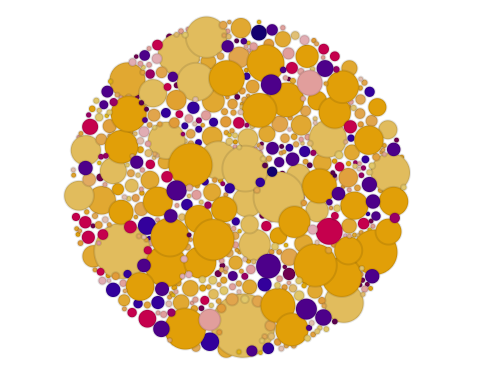
\includegraphics[width=0.5\columnwidth]{force001.PNG}
  \caption{The force graph with default center force. All nodes are attracted to the same center without overlapping each other.}
  \label{fig:force001}
\end{figure}

\begin{figure}
  \centering
  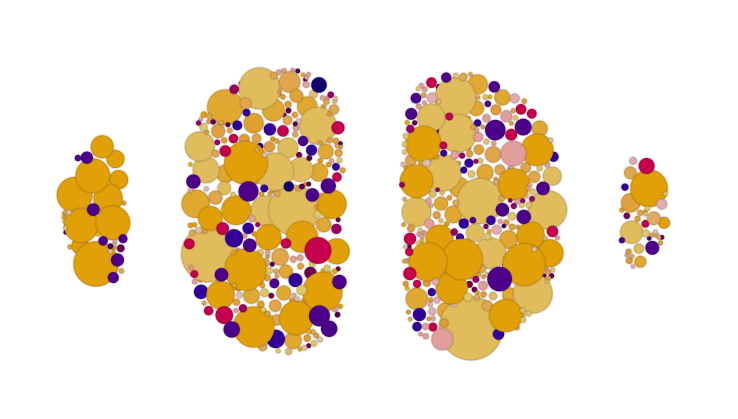
\includegraphics[width=0.6\columnwidth]{force002.PNG}
  \caption{A sample force graph with more than one center force. Having more than one force centers means that different nodes are attracted to their assigned center force.}
  \label{fig:force002}
\end{figure}

\section{Force Graphs -- Real Time Rendered Data Visualizations}

Due to the immense size of D3, the focus of this thesis and its project lies on a rather "small" but quite important part of the library -- the force graph simulation. It is the graph type that is integrated into React as showcased by the thesis project. The visualizations consist of objects that interact with each other in a two-dimensional space. By interacting and moving objects all other objects in the animation are also affected. Figures \ref{fig:force001} and \ref{fig:force002} show an example of D3's force simulation. In figure \ref{fig:force001} there is a single center force that keeps all nodes in the center but also keeps individual nodes from overlapping each other. Force graphs can also be configured to make nodes reject each other even further than their actual size as figure \ref{fig:force004} shows. It is also possible to implement so-called links that also add some complexity to the simulation, as nodes are dependent on each other and not only reject each other but also attract linked nodes as figures \ref{fig:force002} and \ref{fig:force005} shows.

As previously mentioned, all force simulations are calculated, animated, and rendered in the browser which also includes user interaction. The user can, for example, drag nodes around which of course then affect other nodes and the whole simulation as well. Figure \ref{fig:force003} shows well, how dragging one node affects the whole force graph, as all connected nodes follow the dragged node while still rejecting each other and while being attracted to the center force.

\begin{figure}
  \centering
  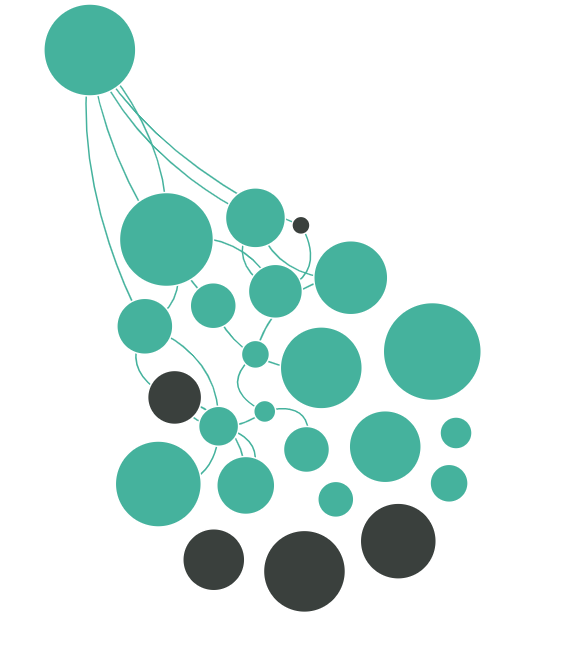
\includegraphics[width=0.4\columnwidth]{forceOwn002.PNG}
  \caption{A sample force graph where the top node is dragged up to the left and the other nodes are dragged along. The force is still keeping the other nodes apart and also drawn to the center though.}
  \label{fig:force003}
\end{figure}

\begin{figure}
  \centering
  
\includegraphics[width=0.45\columnwidth]{forceOwn003.PNG}
  \caption{A sample force graph with one center force. The nodes are configured to reject each other with the function \texttt{r+r/2}.}
  \label{fig:force004}
\end{figure}

D3 provides a somewhat simplified API to be able to quickly implement force graphs in the browser as it can be read in \cite[/d3-force/blob/master/README.md]{D3Github}. The way force simulations work is that developers first have to define or build the simulation. There is a factory method as seen in line 1 of program \ref{prog:simulation} which takes the nodes of the graph as an argument and builds a default simulation. The nodes have to be provided in a particular scheme so D3 can correctly parse the node array. 

\begin{program}
\caption{Code snippets for D3 force simulation code}
\label{prog:simulation}
\begin{JsCode}
simulation.forceSimulation([nodes]) // factory method for a standard force simulation
simulation.tick([iterations]) // called on every tick the simulation goes through
simulation.start() // starts a stopped simulation
simulation.stop() // stops a started simulation
simulation.restart() // restarts a simuliation, resets alpha
simulation.alpha([alpha]) // directly sets alpha value
simulation.alphaTarget([alphaTarget]) // sets alpha target value
\end{JsCode}
\end{program}

\begin{program}
\caption{Sample initialization of a D3 force graph}
\label{prog:d3forceinit}
\begin{JsCode}
const simulation = forceSimulation(data)
  .force('charge', forceManyBody().strength(-150))
  .force('forceX', forceX().strength(0.1))
  .force('forceY', forceY().strength(0.1))
  .force('center', forceCenter())
  .alphaTarget(1)
  .on('tick', ticked)
\end{JsCode}
\end{program}

Another very important aspect of force graphs is the so called "alpha" value system as documented in \cite[/d3-force/blob/master/README.md]{D3Github}, which controls how long the simulation lives. The alpha value is a gradually decaying value that makes the simulation stop if a certain value is reached. Every simulation has a function that is called every "tick" of the simulation as shown in line 2 of program \ref{prog:simulation}. Each tick the alpha value decays via a predefinable function, it happens logarithmically per default. The ticking function takes a handling function will be passed every node position in the simulation which then letsdevelopers link the data to the DOM with D3 again. The tick function will be very important later on when the combination of D3 and React is explained in more detail. Program \ref{prog:d3forceinit} is a simple example that shows how to initialize a D3 force simulation.

\begin{figure}
  \centering
  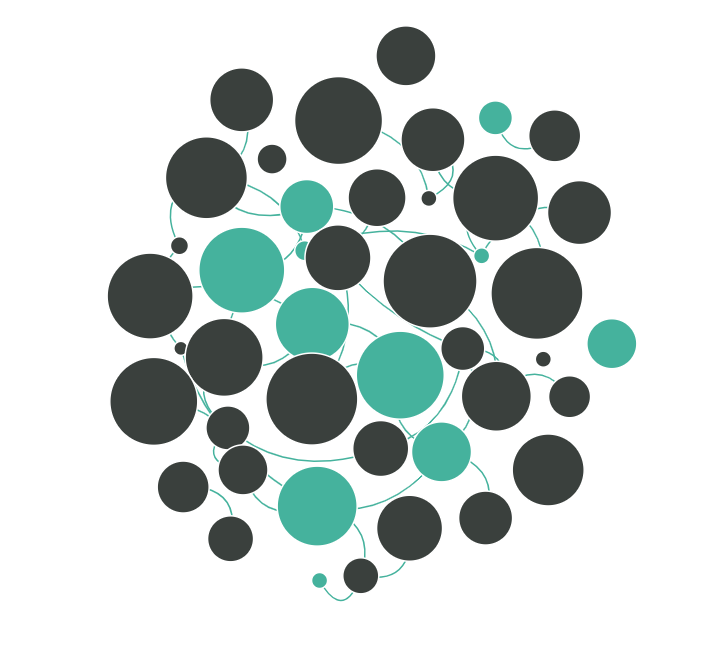
\includegraphics[width=0.45\columnwidth]{forceOwn001.PNG}
  \caption{A sample force graph where some nodes are linked together while still rejecting each other.}
  \label{fig:force005}
\end{figure}

If there is a user interaction, the simulation sometimes has to be restarted or reheated. Programmers can set alpha values and targets to reheat or restart the simulation in case a node is dragged by the user which would possibly require many other nodes in the simulation to react to that user input. That way also the speed of the simulation can be controlled via setting a custom decay function. The documentation in \cite[/d3-force/blob/master/README.md]{D3Github} points to a few methods that can achieve said functionality. The functions on line 3, 4, and 5 of \ref{prog:simulation} can be used to reheat a simulation. Also the functions in line 6 and 7 of \ref{prog:simulation} can be used to set values directly to alter the simulation's life span.

\begin{program}
\caption{D3 written in a fictional functional way}
\label{prog:d3functional}
\begin{JsCode}
const forceParams = compose(
  force('charge', pipe(forceManyBody(), strength(-150))),
  force('forceX', pipe(forceX(), strength(0.1))),
  force('forceY', pipe(forceY(), strength(0.1))),
  force('center', forceCenter()),
)

const simulation = compose(
  forceParams,
  alphaTarget(1),
  on('tick', ticked),
  forceSimulation
)(data)
\end{JsCode}
\end{program}

If a functional approach would be used the code from program \ref{prog:d3forceinit} would look more like in example \ref{prog:d3functional}. The difference between the two code examples in programs \ref{prog:d3forceinit} and \ref{prog:d3functional} might appear to be very subtle, but in reality, it is very significant. By looking closer, it is clear that the variable \texttt{forceParams} is a functional composition of methods that can be reused multiple times in the application. In the first example in program \ref{prog:d3forceinit} the simulation configuration is locked in the function chain. Chaining is a pattern which can easily cause duplicated code in any codebase. 

Writing functional D3 code could also alleviate the confusing unmaintainable code in program \ref{prog:d3confusing} as developers can easily compose repeating DOM manipulation sequences and reuse them throughout the codebase without having to touch code on multiple files in case there is a bug that effects multiple aspects of the application.

\chapter{React – A JavaScript library for building user interfaces}
\label{cha:react}

This chapter introduces the reader to the very popular and widespread front end library called ReactJS. It explains an essential part of React -- its rendering cycle -- which the reader needs to understand at least on a high level to be able to follow upcoming explanations of how the thesis project was implemented. Additionally, the paper elaborates the difference of how React uses declarative code to render data, whereas D3 uses an imperative API to render its data.

\section{Introduction to ReactJS}

The easiest way to find information about React is to visit its official website \footnote{https://reactjs.org}. There is a statement in \cite{React} up front that says: \begin{quote}\begin{english}React is a JavaScript library for building user interfaces.\end{english}\end{quote} which describes React very well. A Facebook engineer called Jordan Walke founded the library in 2011 as presented in \cite[05:30]{ReactFoundingVideo}. Walke wanted to create a tool that would improve the code quality of their internal tool called ''Facebook ads''. Up until then, Facebook continued to develop and use React internally, but since the year 2013, the project is entirely open source. Since the initial open-source release up until now, not only technical engineers of Facebook but also the React open source community itself have been maintaining the library. In late 2017 Facebook even changed React's BSD license to the MIT license, which is even better for the React community, as the MIT license has lesser restrictions than the BSD license.

According to \cite{React} Facebook sees React as a declarative and component-based library. However, a question might come to mind: ''What exactly does it mean for a library to be declarative and component-based?''. The answer to this question might be more straightforward than initially anticipated. In \cite{lloyd1994practical} declarative programming is described as a programming pattern, that expresses the logic of a program without describing its control flow. This means that the actual code only describes what has to be computed not necessarily how it should be done exactly by stating every action explicitly via a function call for example. Declarative programming can be understood as a layer of abstraction, that makes software easier to understand for readers of the code. Declarative programming is therefore very different from the imperative programming pattern described in chapter \ref{cha:d3js}. React's approach of handling the presentation layer is declarative since its API lets developers describe how the application has to look like at any given data variation, which is quite the contrary to D3's API as it can be read in \ref{cha:d3js}. Further information about React's API can be found in section \ref{sec:reactApi} though.

Enabling developers to create a highly component oriented architecture in their software is a fundamental aspect of React as well. Using a component-based library can increase productivity a tremendous amount. However, what does it mean for a library to favor component based architecture? After the initial setup of some boilerplate code, React makes it exceptionally easy to reuse existing components in the codebase to allow even faster development cycles. Once standard input components like buttons or text fields and layout components like page or header components are implemented, they can be reused throughout the whole app; thus significant progress can be achieved in a very short amount of time. Components can be manipulated by passing different properties, which might result in different presentation results of the components. More in-depth information about how React handles components and its props can be found in section \ref{sec:reactApi}.

React components can have multiple applications. There are presentational components for example which are pure functions that simply represent the current application state. Though there are also stateful Components which can hold some application state and react to state changes accordingly via rendering again. React however makes no assumptions about the technology stack that is used in a project as \cite{React} claims. This means that users of the library can decide for themselves if they want to use the built-in state management functionality or if they want to use a third-party library for solving specific problems like global application state for example.

The documentation in \cite[/docs]{React} claims that the library makes use of a so-called ''virtual DOM''. This means that React keeps track of its state data to prevent unnecessary writes to the actual DOM object. JavaScript performs exceptionally well when handling pure JavaScript objects in memory. Keeping the DOM tree of the application in the JavaScript engine's heap as a representation of objects enables React to apply data updates this so-called virtual DOM, then diff the newly applied data with the old tree to then being able to decide what DOM nodes need to be rewritten. Writing or committing to the DOM is the most expensive type of work in the browser, so React tries to keep DOM manipulating actions to a minimum. The React team calls the diffing algorithm ''reconciliation algorithm''. It would go out of the scope of this paper to go more in depth of the algorithm, so it is recommended to read about React's reconciliation algorithm in its documentation \cite[/docs]{React}.

React is a view layer that favors unidirectional data-flow. Every time the application state changes, the whole new data object is passed to React again. As mentioned in \cite[6:50]{ReactFoundingVideo}, the speaker describes the functionality very well via explaining React as a simplified function that could look like this: \texttt{f(data) = UI}. Hence, React can be seen as the view layer that handles presentation as a function of state and data. Once the data has updated the virtual dom, the virtual dom is then passed to React's reconciliation algorithm which then determines if any nodes have to be changed on the real DOM. If there would be a React component that always renders the same \texttt{<div>} with the same data, rendering that very component multiple times would not result in React writing multiple DOM nodes to the browser. The reconciliation algorithm sees that the virtual dom matches the real dom in this case, which results in React not updating the real DOM. Of course, if the component's content is dynamic, the component sometimes has to be re-rendered according to the data changes. If some parts of the data stay the same even after being reapplied to a component, only newly added or removed nodes are committed to the DOM. Even though the reconciliation algorithm prevents expensive DOM operations, the algorithm itself can also be expensive. The documentation in \cite[/docs/optimizing-performance.html\#avoid-reconciliation]{React} advises developers to try to avoid reconciliation to improve performance.

Unidirectional data-flow implicitly means to React, that there is no data binding and no template language. The library only uses \texttt{React.createElement([element])} calls internally, which are hidden behind the so-called ''JSX'' JavaScript language extension. JSX will be explained more i depth in section \ref{sec:reactApi}. As mentioned before, React is just a pure idempotent function of its application state, which means that the same data always produces the same presentation. This also means if the application data has to be changed, a new ''patched'' version of the application data has to be created which then flows into the React render cycle again Unidirectional data-flow is also the reason why React works well with immutable data structures. This paper assumes that the reader knows about immutable data structures, but \cite{ImmutableJS} explains exceptionally well, what are Immutable data structures and how they're used in JavaScript. Going more in-depth on how React works well with immutable state would go out of the scope of this thesis though. It is just essential to know that every time the data change this triggers a whole new render cycle of React. The immutable data structures help React to work out changes in the data structure, as nested data object tree differences can be checked via a cheap equality check when using immutable data structures.

\section{Explaining the React API}
\label{sec:reactApi}

To follow performance discussions and elaborations about the thesis project's prototypes, a general high-level understanding of the API is required. This section introduces the reader to React's public API. The section does not aim to be a tutorial on how to program React applications, but rather to be a high-level explanation of how the API works. Reading this section makes it easy to understand the differences and similarities of React and D3 and how the two libraries play together and how they're also completely different.

\subsection{JSX in general}

\begin{program}
\caption{Creating a React element with JSX} 
\label{prog:reactJsxElement}
\begin{JsCode}
const ReactElement = (
  <div className="hello-world">
    Hello <span className="emph-text">World</span>!
  </div>
)
\end{JsCode}
\end{program}

\begin{program}
\caption{Creating a React element without JSX} 
\label{prog:reactJsxTranspiled}
\begin{JsCode}
const ReactElement = React.createElement(
  "div", 
  { className: "hello-world" }, 
  "Hello ", 
  React.createElement(
    "span", 
    { className: "emph-text" }, 
    "World"
  ), 
  "!"
);
\end{JsCode}
\end{program}

% Notice, that the class property has to be \texttt{className} instead of \texttt{class} as JSX is \emph{not} HTML, but extended JavaScript.

Probably one of the most important aspects of React's API is the JavaScript language extension called ''JSX'' which simplifies the use of React greatly and produces much more readable code. The example in \ref{prog:reactJsxElement} shows an example React component that is written in JSX. When looking at the transpiled output in \ref{prog:reactJsxTranspiled} it is clear how JSX helps to reduce the amount of code and how it greatly improves readablity. The code in \ref{prog:reactJsxTranspiled} also shows that React is just a big composition of \texttt{React.createElement([element])} calls under the hood. When writing JSX code, in reality it is writing declarative code that is just a functional composition of React components. 

Notice, how the createElement function takes up to 3 parameters as documented in \cite[/docs/react-api.html]{React}. The first parameter being the element type (the type can also be a custom user created component or a downloaded third party component), the second parameter being the element's properties and the third parameter being the component's children. In fact, that third parameter makes it possible to compose multiple React components together, as children are nestable. 

Line 2 and 3 in \ref{prog:reactJsxTranspiled} show, how a React element is created. A node of type \texttt{''div''} is created and the property \texttt{\{className: ''helo-world''\}} is passed. Each parameter after Line 3 is a child of the created \texttt{<div>} node. The React element has 3 children which is demonstrated by the code example where the element is written in JSX in \ref{prog:reactJsxElement}. First, there is the string ''Hello '', then there is a \texttt{<span>} which also has children, and finally there is the exclamation mark string at the end. When going back to the transpiled code example in \ref{prog:reactJsxTranspiled}, lines 4 to 10 exactly show what kind of children are passed to React's element creating function. Notice, that the class property has to be ''className'' in JSX instead of ''class'' because JSX is \emph{not} HTML, but extended JavaScript. Something also worth looking at is line 5 in \ref{prog:reactJsxTranspiled}. A nested \texttt{createElement()} call shows, how components can be composed together.

Because JSX is a language extension, a transpilation step is needed in order to produce production code. The common tool to use is called ''Babel''. There is a caption in \cite{Babel} that says: \begin{quote}\begin{english}Use next generation JavaScript today.\end{english}\end{quote} The documentation in \cite[/docs/en]{Babel} explains, how modern JavaScript features can be used in any JavaScript project. The code which includes those modern features is normalized and transpiled by Babel to also work in older browsers. The tool accomplishes this by transforming the JavaScript code via its core implementation but also via some third party plugins. A babel plugin has been created to transform JSX components into the syntax that can be seen in the code in \ref{prog:reactJsxTranspiled}. Just as a sidenote, altough JSX became popular in conjunction with React, there are also other web technologies that make use of JSX like Vue.js \footnote{https://vuejs.org/} for example.

\subsection{Explaining React components}
\label{sec:reactComponents}

\begin{program}
\caption{Simple example of a React component and its usage} 
\label{prog:reactHelloWorld}
\begin{JsCode}
const HelloComponent = props => {
  const name = props.name;
  return <div>Hello World to {name ? name : "you"}!</div>;
};

const PageComponent = props => {
  props.customFn("I get passed to the handler function!");
  return (
    <div>
      <h1>{props.title}</h1>
      <div>{props.content}</div>
      here are my children: [{props.children}]
    </div>
  );
};

const App = () => {
  return (
    <PageComponent
      customFn={console.log}
      title="I render the title prop"
      content="I render the content prop"
    >
      <HelloComponent />
      <HelloComponent name={"Max"} />
    </PageComponent>
  );
};
\end{JsCode}
\end{program}

As mentioned before, React is a highly component oriented web technology. The example code in \ref{prog:reactHelloWorld} includes a sample presentational component called ''HelloComponent'' on line 1, a page layout component on line 6 and the base App component on line 17. The app renders the page layout coponent, passes a few props and then renders the HelloComponent twice inside the layout component. One time the HelloComponent receives the prop \texttt{name} and one time the property is omitted. The output of the hello world example can be seen in figure \ref{fig:reactHelloWorld}. The example in \ref{prog:reactHelloWorld} visualizes, how components can be reused throughout the application with different configurations and in different arrangements. The page layout component could be declared in its own file to be reused in every page of the app. Via props React provides a solid mechanism to control static state of the components that receive the props. 

It is of utmost importance to understand, that props -- once they're passed to a component -- are static and immutable inside the receiving component. Components that render props can be seen as pure functions that only render the props that they receive each render cycle. The props could thus be understood as the parameters of the pure functions.

\begin{figure}
  \centering
  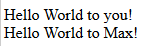
\includegraphics[width=0.35\columnwidth]{react001}
  \caption{React hello world sample output}
  \label{fig:reactHelloWorld}
\end{figure}

\begin{program}
\caption{Simple example of a React component and its usage} 
\label{prog:reactStatefulComponent}
\begin{JsCode}
const Count = props => (
  <div>
    <div>I render the count</div>
    <div>The count is currently {props.count}</div>
  </div>
);

class StatefulComponent extends React.Component {
  state = {
    count: 1
  };

  counterHandler = () => {
    this.setState(state => ({ count: state.count + 1 }));
  };

  render() {
    return (
      <div>
        <Count count={this.state.count} />
        <button onClick={this.counterHandler}>+1</button>
      </div>
    );
  }
}

const App = () => <StatefulComponent />;
\end{JsCode}
\end{program}

\begin{figure}
  \centering
  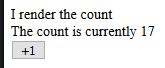
\includegraphics[width=0.25\columnwidth]{react002}
  \caption{React counter component output}
  \label{fig:reactCounterComponent}
\end{figure}

% what is state for the one component is immutable static prop for the other

%Another important aspect of React which is important for this project are its life cycle methods. Each component has a life cycle that will be executed on each rendering cycle. Developers can hook into those life cycle methods to implement some logic that should be executed after a component mounts or after a component was updated for example. The most well known life cycle methods of React are \texttt{componentDidMount()} or \texttt{componentDidUpdate()}.

% talk about animating stuff in react

\section{The difference between imperative and declarative APIs}



\chapter{Data Visualization}
\label{cha:visualization}

\section{Introduction to force graphs}

\section{Prototypes}

\subsection{Pure D3 prototype}

\subsection{Pure React prototype}

\subsection{D3 and React hybrid}

\section{Comparison of the different proposed Prototypes}

\section{Building a stable Testing Environment}

\section{Testing methodologies}

\section{Testing devices}

\chapter{Performance Testing and User Perception}
\label{cha:performance}

The research question of the thesis is if React can be combined with D3 without losing any performance in the browser. The following sections introduce the reader not only to the benchmark setup and testing methodologies but also to the final results of the benchmarks. There is also a discussion which elaborates all test results. Since humans cannot measure the exact amount of frames per second, a special section introduces the reader to the human perception of fluid animations and how the testing results can be interpreted even further with that knowledge.

\section{Test Environment Setup}

This section describes the testing environment that was implemented to compare the three force simulation component prototypes. There are a few challenges that had to be taken into account when realizing the testing environment. Also, the implementation details are elaborated and explained. Last but not least, the testing devices are introduced which are used to run the benchmark.

\subsection{Challenges}

One of the most challenging aspects of the thesis project is the performance measurement of the prototypes. Modern browsers have an uncountable amount of features that help to smooth out the performance to improve user perception. Getting some consistent performance numbers is much harder due to inconsistent browser optimizations. Using different browsers for benchmarks also means that different JavaScript runtimes are used to run the benchmarks. All engines have different execution and parsing speeds. Also, the mechanism to speed up frequently accessed script code is different, which also makes it harder to get consistent performance numbers.

When benchmarking web applications, it is very complicated to get performance values that have scientific relevance, which can be compared to get some accurate research results. The next section introduces a system that was primarily implemented to measure the performance of JavaScript web applications. The system tries to tackle all challenges to produce detailed benchmark results.

Another big problem is the fact that browsers detect the refresh rate of monitors when utilizing the request animation frame functionality. Monitors with a refresh rate of 144 Hertz allow browsers to produce up to 144 frames per second. 60-Hertz monitors, on the other hand, limit the browser's framerate to 60 FPS. The maximum amount of animation frame executions in any browser can only ever go up to the monitor's amount of Hertz the browser window is running in. 

Speaking of utilizing the request animation frame functionality, it must be mentioned that each browser has a different implementation of the functionality. The Chrome\footnote{\url{https://www.google.com/intl/de/chrome/}} browser, for example, is smoothing out the performance by trying to executing animation frames regularly, which means that the overall performance might be lowered to achieve a smoother framerate as explained in \cite{ChromeRAF}. Experience shows that Firefox\footnote{\url{https://www.mozilla.org/de/firefox/new/}}, on the other hand, always fires its animation frames whenever a frame is available, which can result in higher overall but not as consistent framerates.

Last but not least, another challenge was to build a performance measuring environment that can be used without adding code to the prototypes. Theoretically, each prototype should be a complete component that can be shipped as a third party library. By adding performance measurement specific code, the components would contain functionality that is not needed when shipping production builds of the components.

\begin{figure}
  \centering
  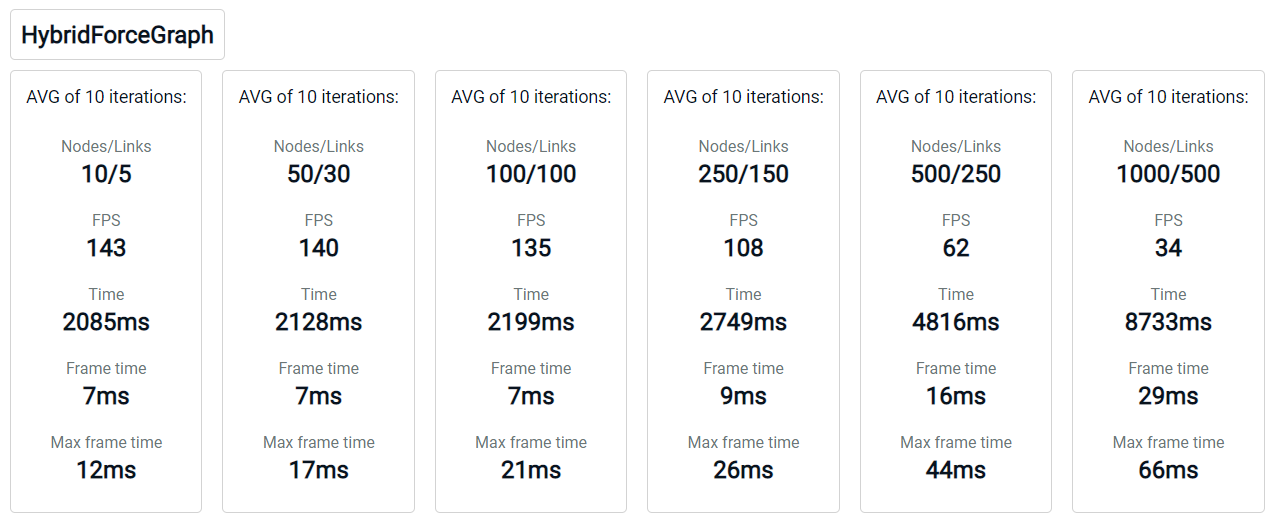
\includegraphics[width=1\columnwidth]{testresults}
  \caption{Hybrid prototype benchmark results.}
  \label{fig:reactD3benchResult}
\end{figure}

\subsection{Building a Stable Testing Environment}
\label{sub:perfImplDetails}

A testing environment which produces consistent data input across multiple iterations yields the best testing results when benchmarking all three prototypes. Testing the force simulation prototypes with the same data across multiple benchmarks, environments, and devices is of utmost importance. A valid solution is to use a pseudo-random data generator which can be restarted and reseeded each benchmark iteration.

Generating an arbitrary amount of random node and link positions is not a problem, as JavaScript has a built-in random generator which can be utilized to generate random data. Unfortunately, JavaScript's random generator cannot be seeded to achieve consistent pseudo-random results. The library \emph{seedrandom} in \cite{SeedRandom} is the perfect technology to solve the problem of generating consistent data across multiple iterations of the benchmark tests.

Since browsers frequently yield different performance numbers across iterations with identical data, the amount cycle per test data iterations sets has to be increased. When testing one specific iteration multiple times, the average value has much more significance than testing an iteration only once. Therefore the testing environment must have support for different iteration configurations, which can be run an arbitrary amount of times.

\begin{figure}
  \centering
  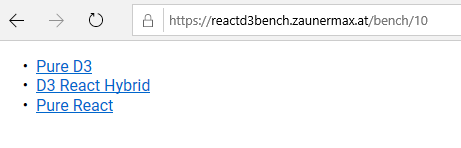
\includegraphics[width=0.5\columnwidth]{reactd3bench}
  \caption{Overview of the benchmark application.}
  \label{fig:reactD3bench1}
\end{figure}

The testing environment is designed to be a stateful container which generates some random data and then passes it to the desired prototype. D3 simulations provide a mechanism to add an event handler whenever the simulation stops. It is, therefore, no problem to pass a handler to the benchmark component that is executed whenever the simulation stops. The handler can be used to restart the benchmark with some newly generated data until the desired amount of benchmark iteration cycles is reached.

Pseudo-random generated data is obtained by a specially implemented custom helper utility module. The custom module is designed to generate a specified amount of random nodes and links. The method to generate random data takes two parameters---the number of nodes and the number of links. Generating consistent pseudo-random data is possible by internally using the previously mentioned seedrandom module.

Tackling the performance measurement problem is a much harder task, however. To be able to measure the number of frames per second, the request animation browser functionality can be used. Another custom implemented module provides some functionality that is specifically designed to measure performance intensive JavaScript animations. By requesting an animation frame as often as possible in a terminable infinite loop, a reference timestamp can be used to measure the amount of animation frame executions per seconds which is equal to the frames per second the browser produces.

Presenting the performance results must not be underestimated either. To provide benchmark results appealingly, each iteration is represented via a visual container that contains all relevant information for a specific test iteration. If there are six test iterations, six containers are rendered after the benchmark. The containers contain the number of cycle per iteration, the test configuration, the number of frames per second, the overall execution time per cycle, the average frame time, and also the highest frame time. Figure \ref{fig:reactD3benchResult} shows how the benchmark results visually look like.

Finally, the benchmark tool has to be easy to use on all kinds of devices. The thesis project also contains a small React application which can be deployed on any static web hosting service that can serve single page applications. A visual representation of the basic benchmark app can be seen in figure \ref{fig:reactD3bench1}. The React application is a wrapper around the testing environment, which lets users select the desired benchmark for any of the three force simulation prototypes and then runs it in the browser. Each benchmark also has an easily distinguishable URL to be able to copy paste a specific benchmark URL into any browser. Figures \ref{fig:reactD3bench1} and \ref{fig:reactD3bench2} show how the URL contains all relevant benchmark parameters. That way the benchmark URLs can be pasted into any browser to execute the benchmark. 

\begin{figure}
  \centering
  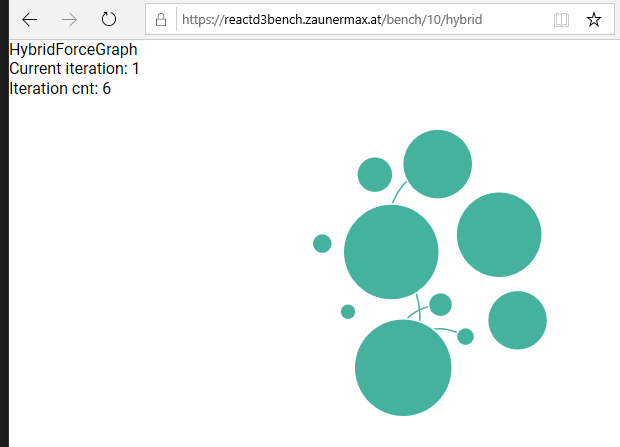
\includegraphics[width=0.6\columnwidth]{reactd3bench1}
  \caption{The benchmark currently iterating through hybrid prototype iterations.}
  \label{fig:reactD3bench2}
\end{figure}

\section{Testing Setup}

Having a bulletproof testing setup plays a fundamental role in producing scientifically releveant test results. Therefore, the following sections of the thesis provide a thorough insight on the testing devices and on how the whole benchmark methodology is conceptionalized. 

\subsection{Testing Devices}

\begin{table}
  \centering
  \begin{threeparttable}
    \caption{The table shows a list of low-end testing devices.}
    \label{tab:lowendTestingDevices}
    \centering
    \def\rr{\rightskip=0pt plus1em \spaceskip=.3333em \xspaceskip=.5em\relax}
    \setlength{\tabcolsep}{1ex}
    \def\arraystretch{1.20}
    \setlength{\tabcolsep}{1ex}
    \small
    \begin{english}
      \begin{tabular}{|c||c|c|c|}
        \hline
          \multicolumn{1}{|c||}{\emph{Device}}&
          \multicolumn{1}{|c}{\emph{CPU}} &
          \multicolumn{1}{|c}{\emph{GPU}} &
          \multicolumn{1}{|c|}{\emph{RAM}} \\
        \hline
        \hline
        OnePlus 1 & 
        Snapdragon 801 & 
        Adreno 330 & 
        3GB \\
        \hline
        OnePlus 5T & 
        Snapdragon 835 & 
        Adreno 540  & 
        8GB \\
        %%\hline
        %%Samsung G\tnote{1} \hspace{0.1mm} S8 & 
        %%Exynos 8895 & 
        %%Mali-G71 MP20 & 
        %%4GB \\
        %%\hline
        %%Samsung GT\tnote{2} \hspace{0.1mm} A10.1 &
        %%Exynos 7870 & 
        %%Mali-T830 MP2 & 
        %%3GB \\
        \hline
        SurfaceBook & 
        Intel i5-6300U & 
        Intel HD 520 & 
        8GB \\
        \hline
      \end{tabular}  
    \end{english}
    %%\begin{tablenotes}
    %%\item [1] Galaxy
    %%\item [2] Galaxy Tab
    %%\end{tablenotes}
  \end{threeparttable}
\end{table}

The amount of test devices should be as high as possible while still being reasonable regarding to the effort it takes to process all resulting benchmark data. A total amount of six devices is enough to retrieve scientifically significant results. The range of devices is divided into two sections: high-end devices and low-end devices. 

The mobile devices used for testing are a OnePlus 1 phone, a OnePlus 5t phone, and a SurfaceBook in tablet mode. All low-end devices and their specs are listed in table \ref{tab:lowendTestingDevices}. It must be noted that every selected low-end device has a monitor refresh rate of 60-Hertz. 

The table \ref{tab:highendTestingDevices} introduces all high-end devices which have a monitor refresh rate of 144-Hertz. Two of the listed devices are custom tower builds with custom specs and one device is a the Razer Blade 15 laptop with specs defined by its manufacturer. All in all the devices should provide a good overview of the performance of the force graph components.

\begin{table}
  \centering
  \begin{threeparttable}
    \caption{The table shows a list of high-end high refresh rate testing devices.}
    \label{tab:highendTestingDevices}
    \centering
    \def\rr{\rightskip=0pt plus1em \spaceskip=.3333em \xspaceskip=.5em\relax}
    \setlength{\tabcolsep}{1ex}
    \def\arraystretch{1.20}
    \setlength{\tabcolsep}{1ex}
    \small
    \begin{english}
      \begin{tabular}{|c||c|c|c|c|}
        \hline
          \multicolumn{1}{|c||}{\emph{Device}}&
          \multicolumn{1}{|c}{\emph{CPU}} &
          \multicolumn{1}{|c}{\emph{GPU}} &
          \multicolumn{1}{|c|}{\emph{RAM}} \\
        \hline
        \hline
        Tower (Max Z.) & 
        Intel i9-7900X & 
        2x Nvidia GTX 1080Ti & 
        32GB \\
        \hline
        Razer Blade 15 (2018) & 
        Intel i7-8750H & 
        Nvidia GTX 1070 Max-Q  & 
        16GB \\
        %%\hline
        %%Tower (Max J.) & 
        %%Intel i7-7700k & 
        %%Nvidia GTX 1070 & 
        %%16GB \\
        \hline
        Tower (Patrick M.) &
        Intel i7-6700k & 
        Nvidia GTX 1080 & 
        16GB \\
        %%\hline
        %%Tower (Julian J.) & 
        %%Intel i7-7700k & 
        %%Nvidia GTX 1070 & 
        %%16GB \\
        \hline
      \end{tabular}  
    \end{english}
  \end{threeparttable}
\end{table}

\subsection{Testing Methodologies}

\begin{figure}
\centering
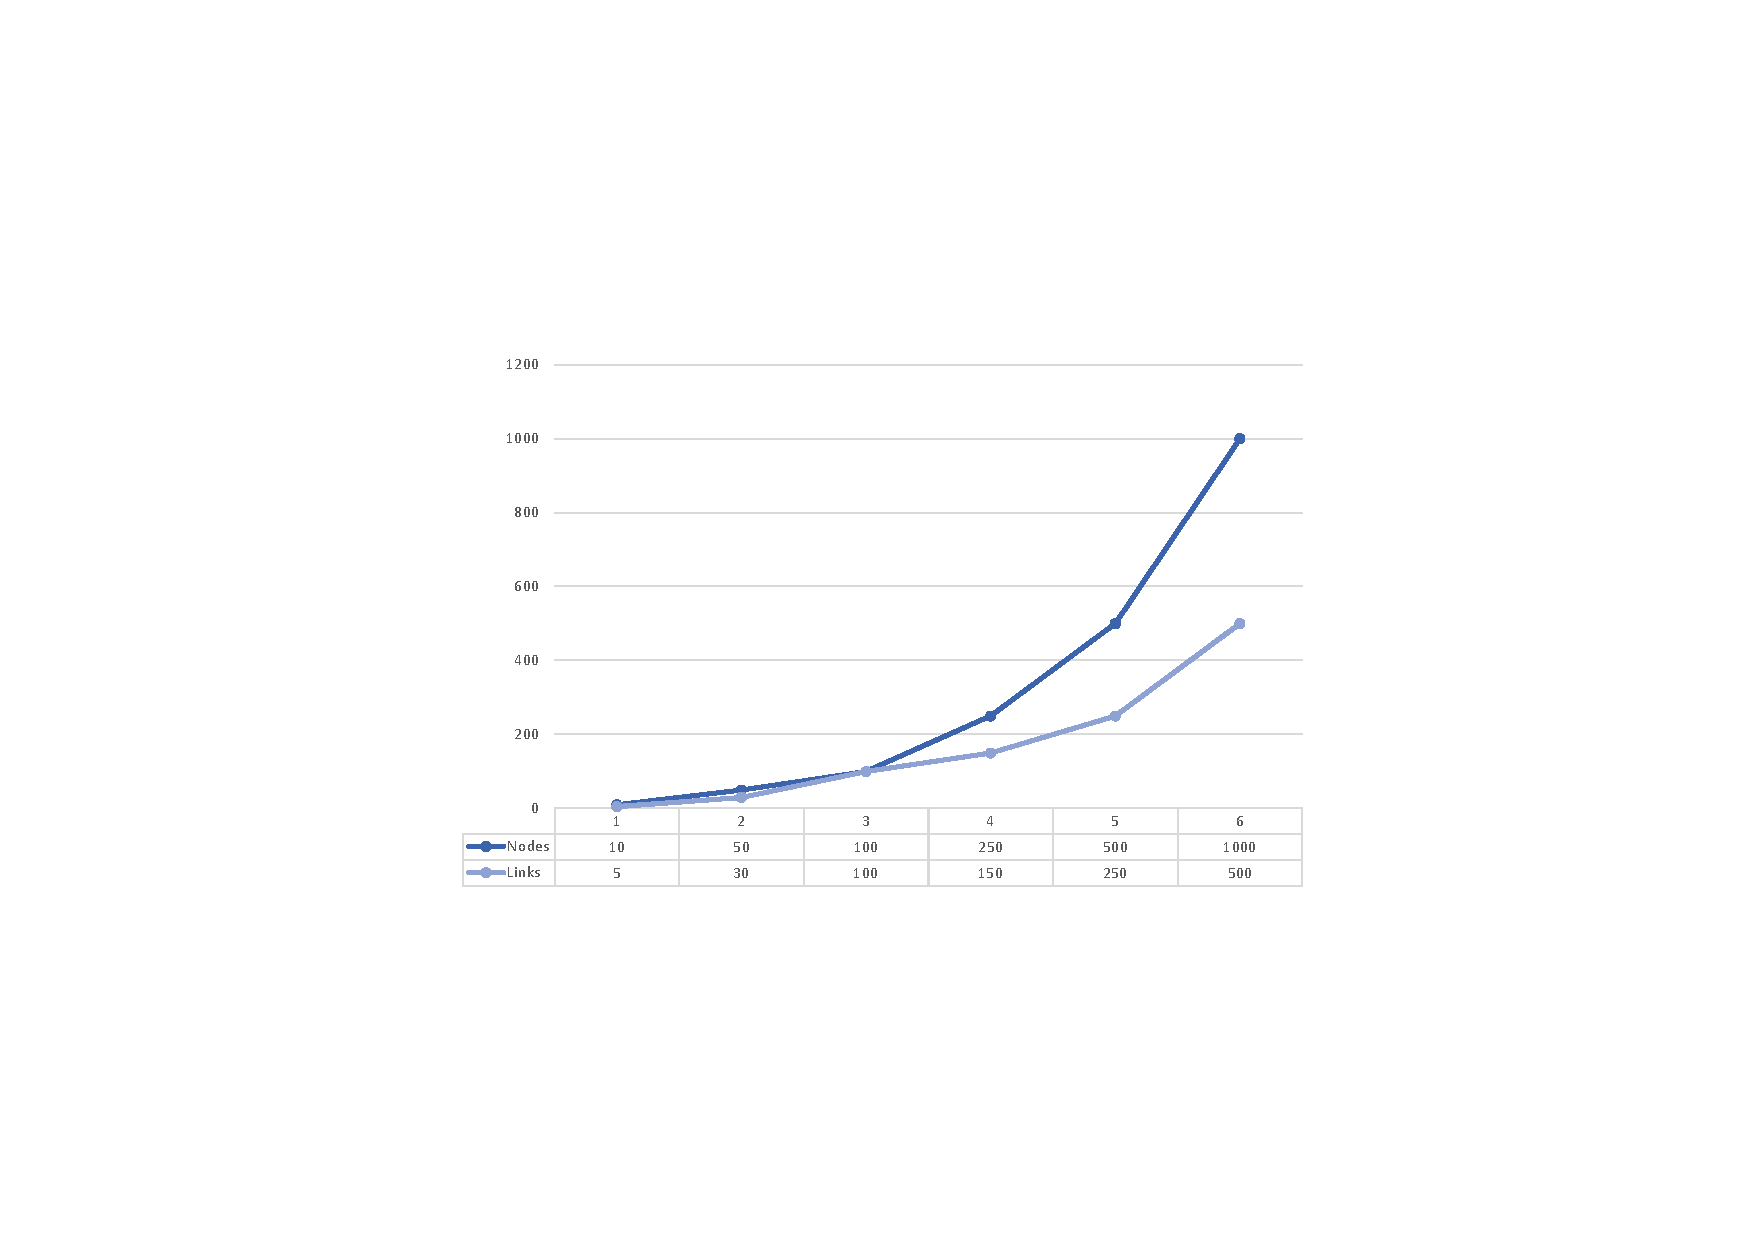
\includegraphics[scale=2.5, trim= 4cm 5cm 4cm 5cm, clip, width=1\columnwidth]{perfIterations.pdf}
\caption{Benchmark iteration configuration.}
\label{fig:perfIterations}
\end{figure}

Running the benchmarks to get valid and scientific testing results is relatively straight forward. To get the most declarative performance numbers it is best to mainly use devices with a high monitor refresh rate. Devices with a low monitor refresh rate can possibly falsify some testing results. If, for example, a browser could possibly render 100 frames per second on an iteration, a system with a 60-Hertz monitor would only be able to measure a maximum of 60FPS as the theoretically possible 100 FPS would be capped to the monitor's 60-Hertz refresh rate.

Devices with high refresh rates can be sufficient for measuring the overall best performing prototype. One of the more interesting research aspects of the thesis though is the question, how well the prototypes perform on mobile devices with lower performance specifications than desktop PCs. Thus the testing results must be split up into different categories as a consequence. Due to the fact that not only frames per second, but also other perfromance aspects like total execution time are measured, the lower performing devices can also be compared to each other.

Each device runs through six iterations per prototype with exponentially increasing render difficulty. Figure \ref{fig:perfIterations} shows the benchmark configuration for the benchmark. Starting with a node count of 10 and a link count of five, the configuration ultimately goes up to 1000 nodes and 500 links. The third iteration is special, as the number of nodes and links is the same. The special configuration was added to test an extreme scenario of all nodes being connected to each other to induce some extra performance heavy force calculations.

Each iteration runs through 10 cycles which equals a grand total of 60 cycles per prototype, browser, and device combination. Three high-end devices with 144-Hertz monitors and the three low-end devices with 60-Hertz monitors run the benchmark iterations in the Chrome and in the Firefox browser. The two browsers were selected, because they are the most significantly used, platform independent browsers worldwide according to the statistics in \cite{StatCounterBrowserMarketShare} and \cite{W3CBrowserMarketShare}. Taking into account that there are six devices, three prototypes, and two browsers, the total number of iterations is 36 and the total number of iteration cycles is 360 as every iteration has 10 cycles.

\section{Benchmark Results}

This section answers the research question if React can be combined with D3 without introducing any performance losses in the browser. Extensive benchmark testing sessions resulted in some remarkable research results which are presented below. After presenting the test results, an introduction to the human perception of fluid animations helps the reader to follow the subsequent interpretation of the benchmark results.

\subsection{Introducing the Test Results}

First of all, the thesis project is a success, as the overall performance numbers show a clear trend that the hybrid prototype is ahead of Uber's pure react implementation. The total execution time of all combined benchmark iteration cycles is exactly 25326ms when combining the average execution times of each test. When converting milliseconds to hours, the result is 7.04 hours. Since the benchmark environment was designed for extensive benchmark sessions, the time between running the benchmarks was minimized. The only tedious and most time-consuming task was to write down the actual benchmark results. Letting devices run the tests required no further user interaction. 

Starting with the low-end devices, figure \ref{fig:perfLowEnd001} shows the average FPS of the low-end devices. An overall downwards trend can immediately be seen in the FPS chart, which is expected, of course. The more DOM nodes the browsers have to calculate, the lower the frames per second get per iteration. Each group of bars in the chart represents an average value for each prototype per benchmark iteration. Note that all values are the average taken from 10 iteration cycles of the Chrome and the Firefox browser. The prototypes mostly yielded the expected performance numbers starting with the reference performance of the pure D3 prototype, followed by the hybrid component and then finally followed by the pure React force graph component.

\begin{figure}
\centering
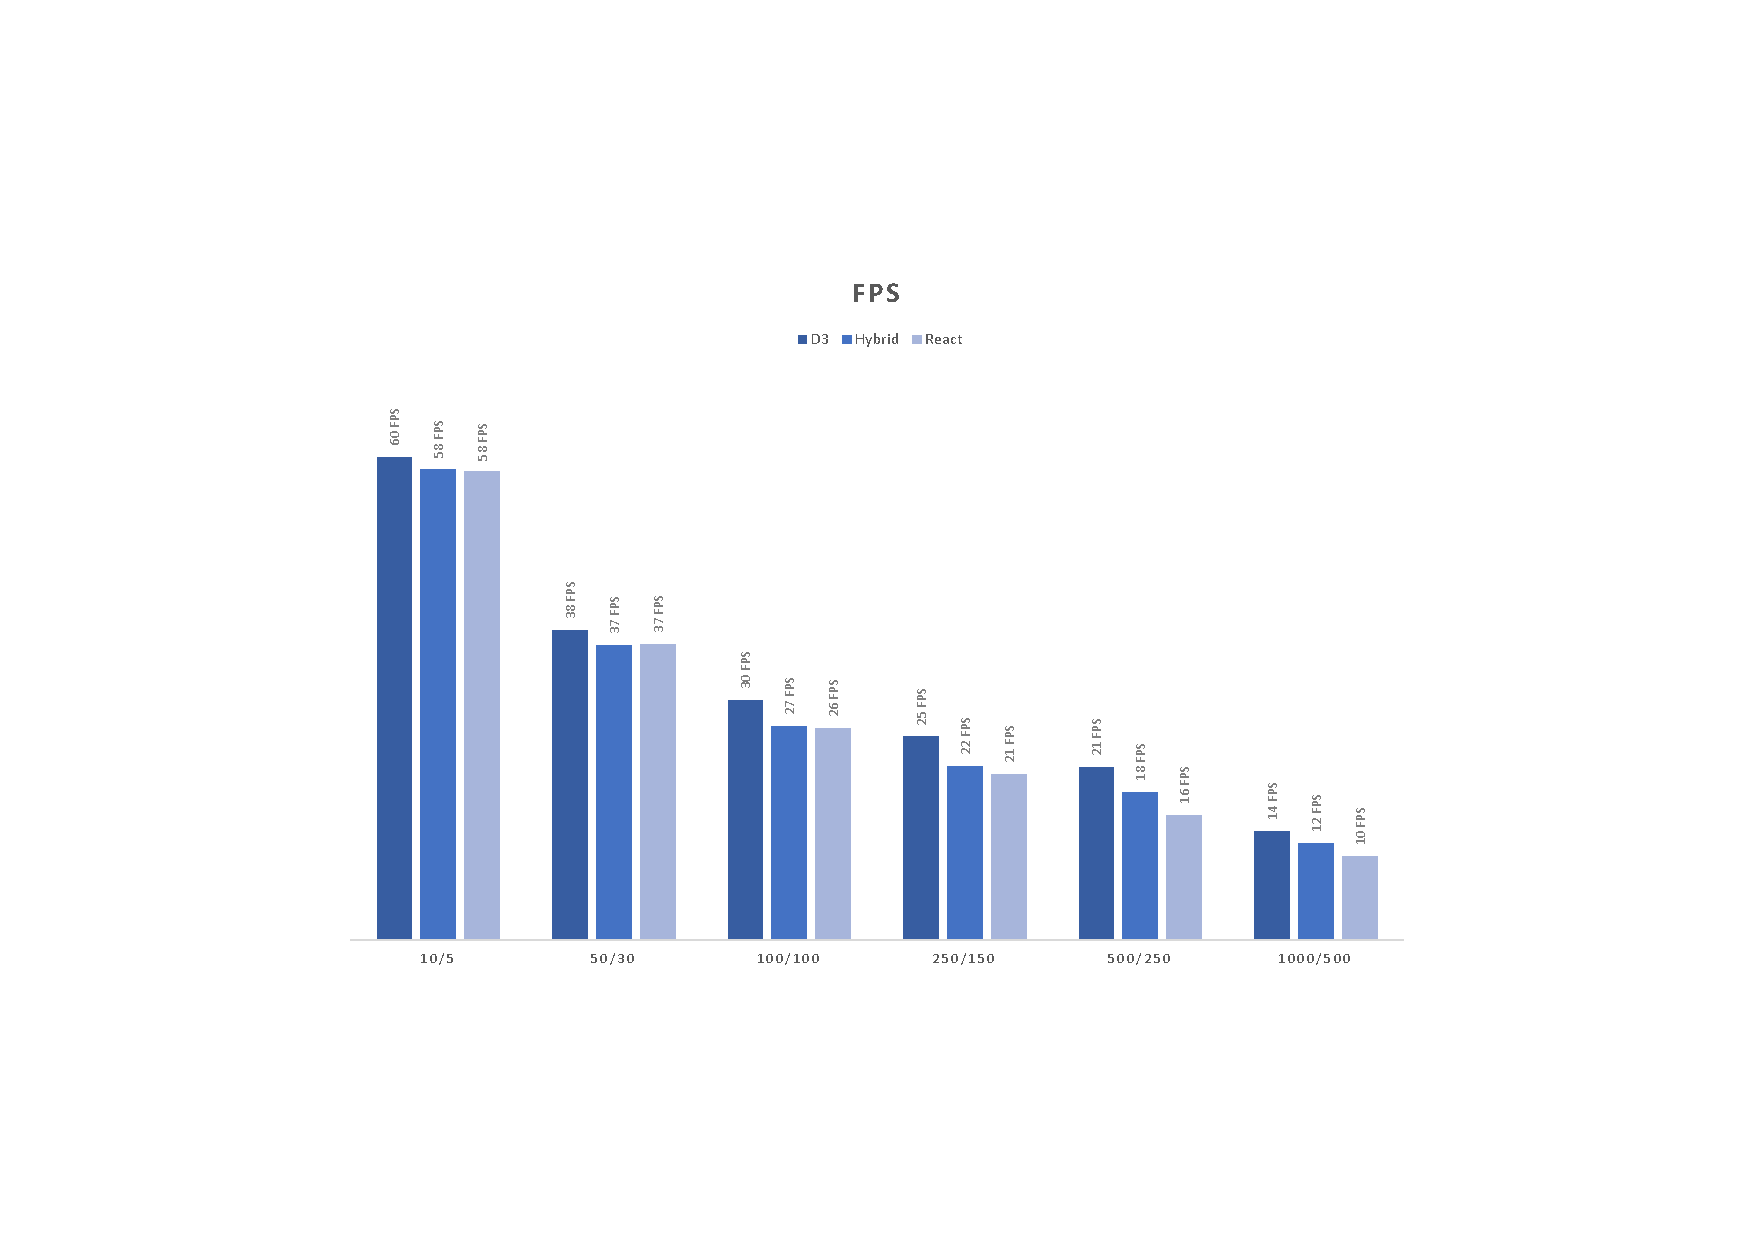
\includegraphics[scale=2.5, trim= 4cm 4.5cm 4cm 4.5cm, clip, width=1\columnwidth]{perfLowEnd001.pdf}
\caption{Low-end devices' average frames per second per benchmark iteration cycle (higher is better).}
\label{fig:perfLowEnd001}
\end{figure}

Following up with the high-end devices, figure \ref{fig:perfHighEnd001} shows the average FPS values of the high-end benchmark iterations. Looking at the bar chart, it is apparent that the high-end devices hit the FPS cap of 144FPS throughout the first few iteration cycles. As mentioned before, the devices would have been able to put out a higher number of frames per second but were limited to the browsers animation frame functionality which is in itself limited to the devices' monitor refresh rate. When looking at the third iteration, a steady decrease of FPS can be observed though, as the iteration difficulty is high enough for all devices not to hit the monitor refresh rate limit anymore.

\begin{figure}
\centering
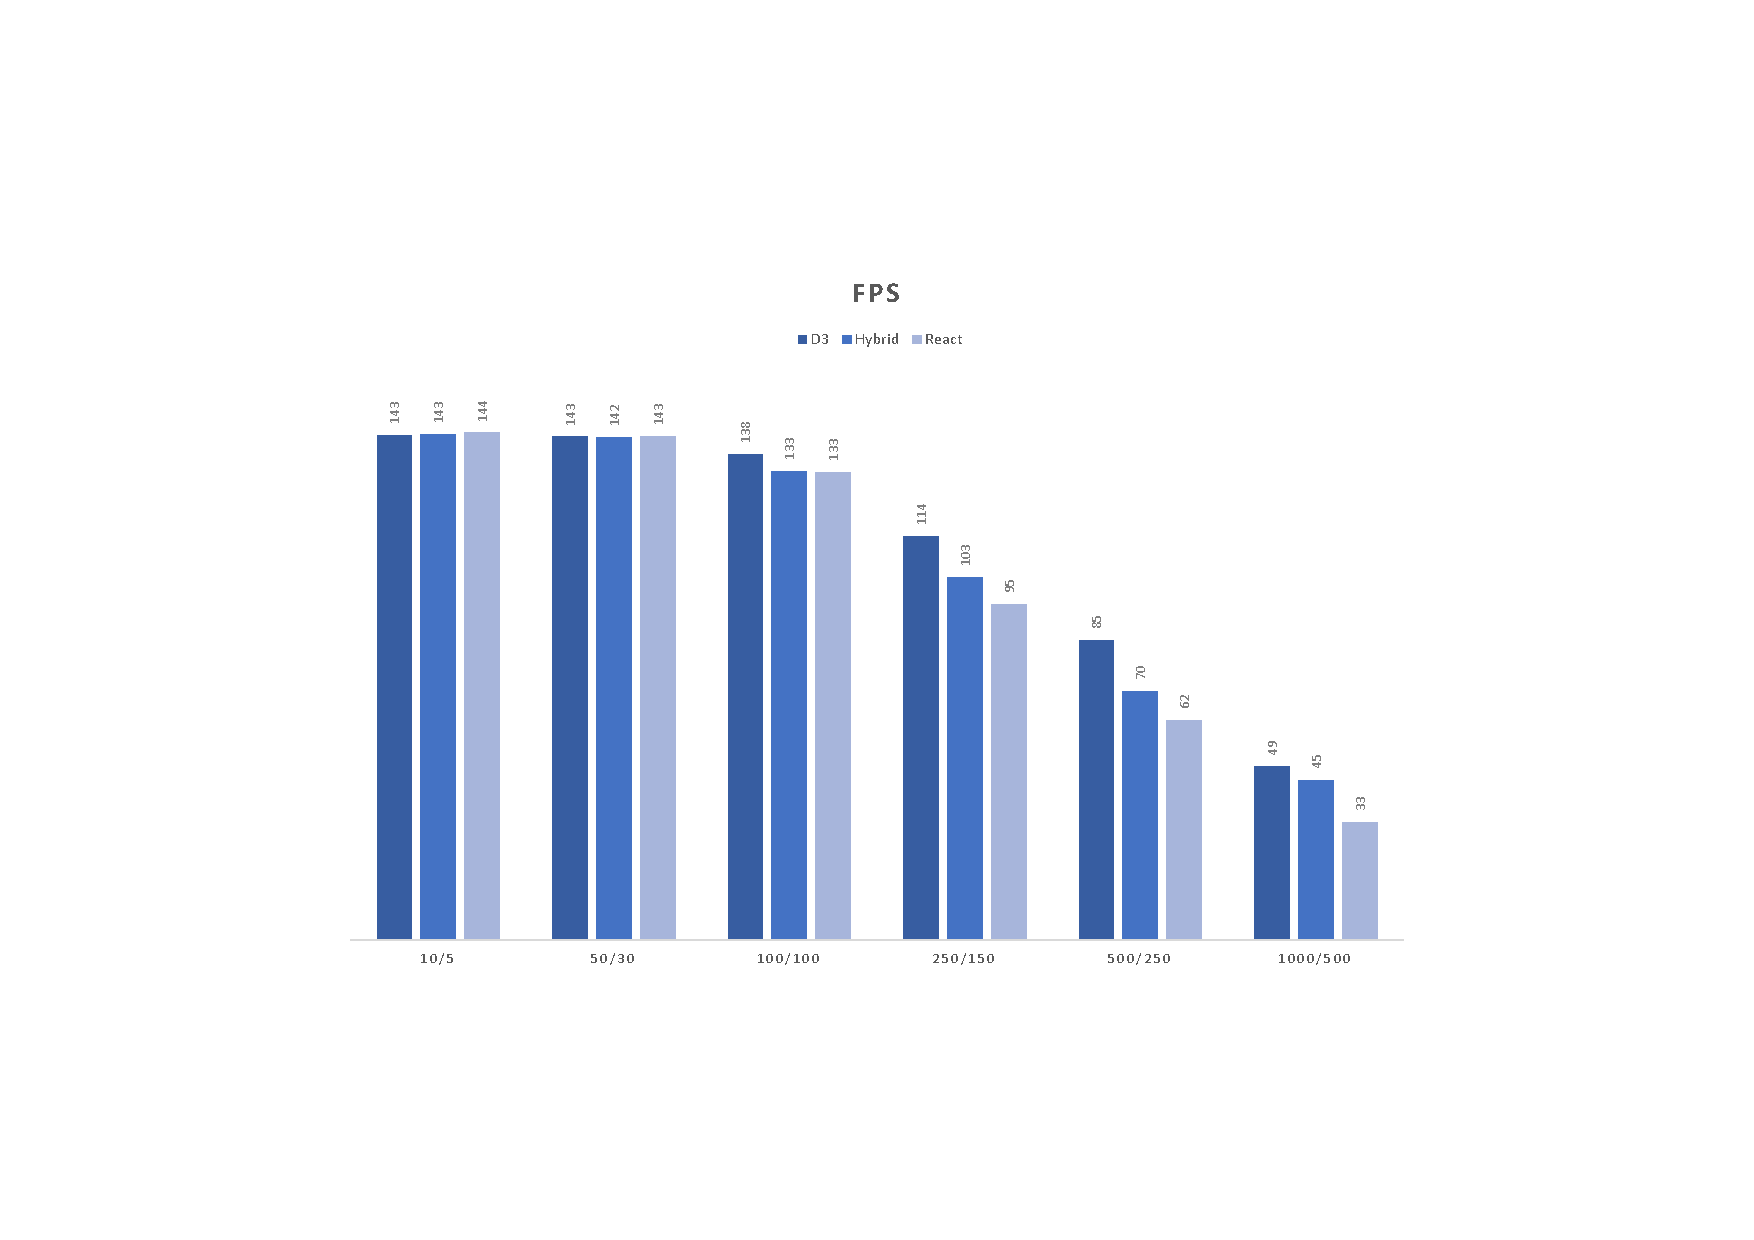
\includegraphics[scale=2.5, trim= 4cm 4.5cm 4cm 4.5cm, clip, width=1\columnwidth]{perfHighEnd001.pdf}
\caption{High-end devices' average frames per second per benchmark iteration cycle (higher is better).}
\label{fig:perfHighEnd001}
\end{figure}

The bar chart in figure \ref{fig:perfLowEnd002} shows the average time it took to complete the benchmark fully. Via the browsers' performance API, exact timestamps can be measured once a benchmark cycle starts, and once it ends. By subtracting the start timestamp from the end timestamp the overall time to execute is calculated. Like the FPS chart, the time to complete chart also shows all average values it took the different prototypes to complete the benchmark cycles fully.

\begin{figure}
\centering
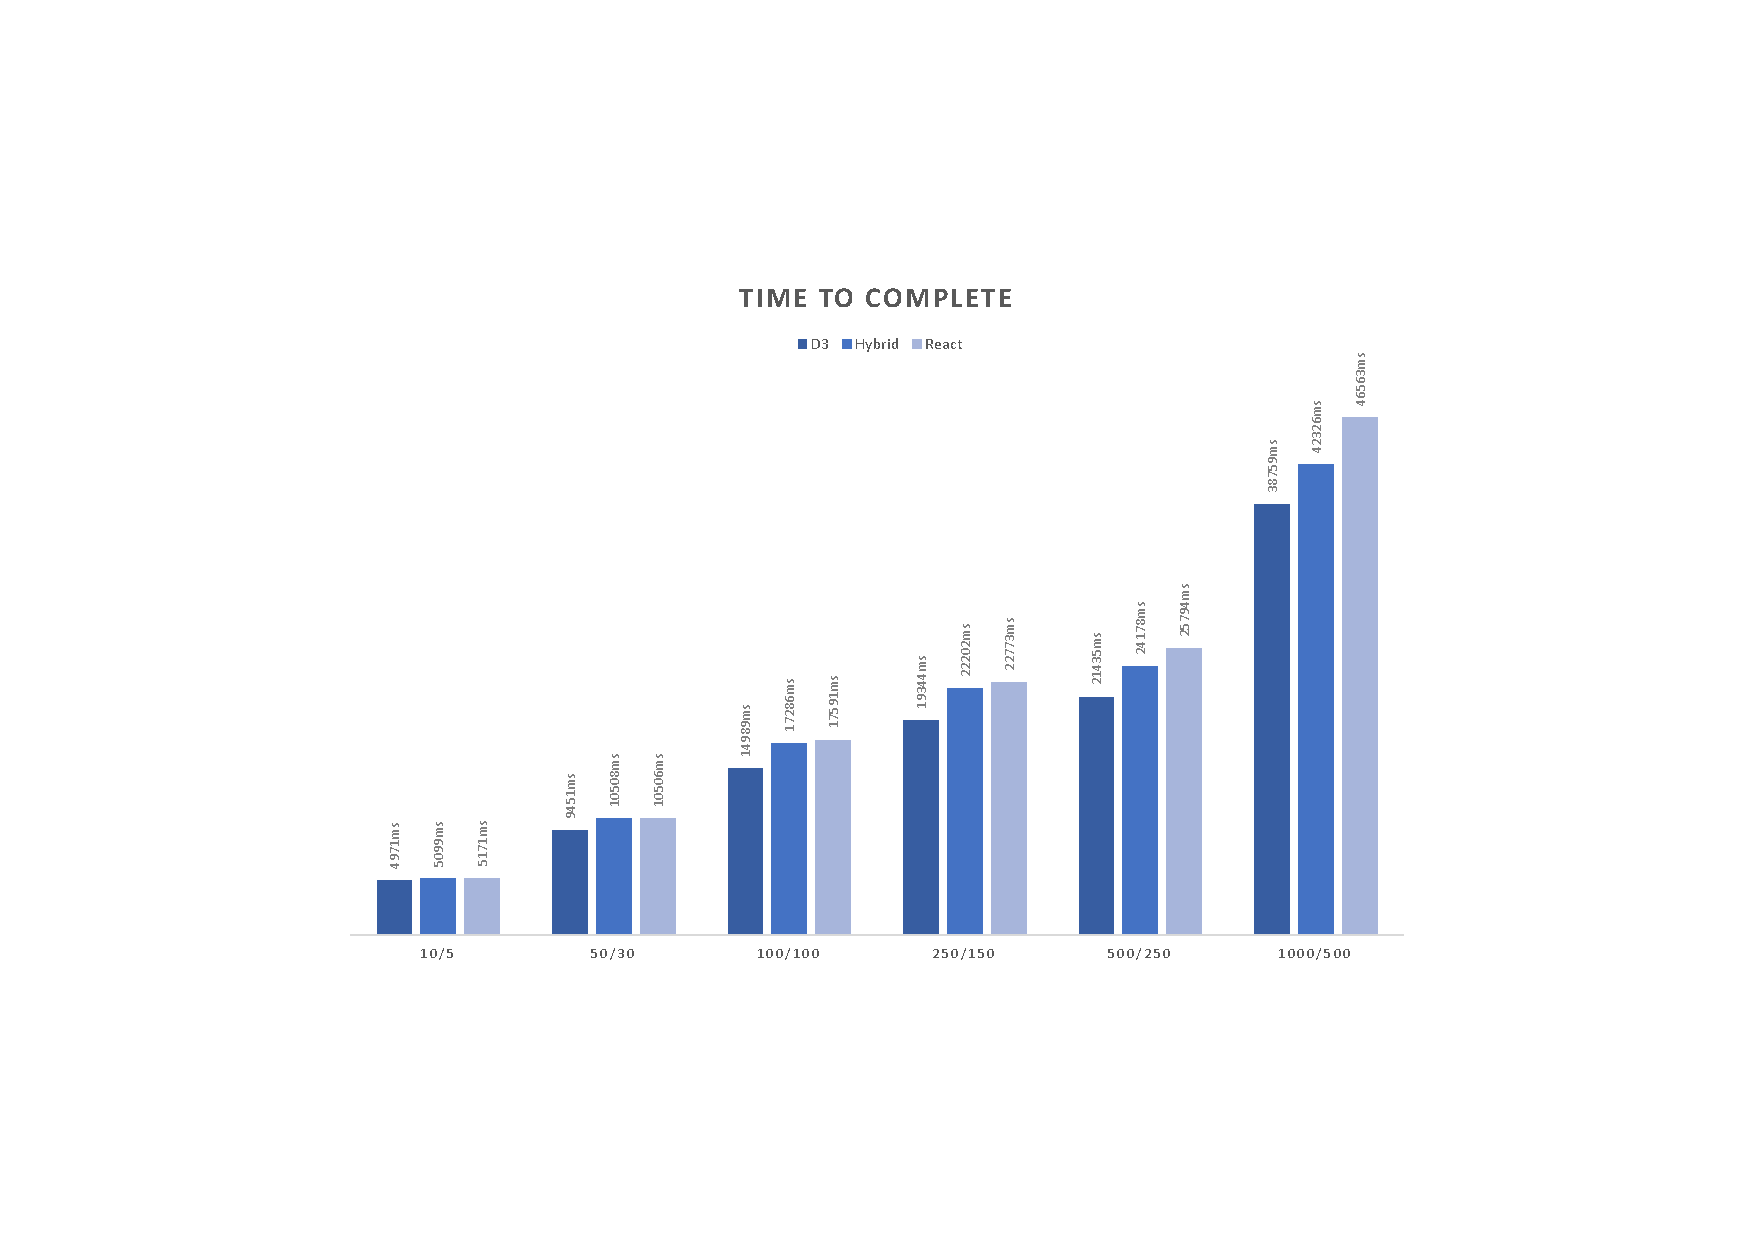
\includegraphics[scale=2.5, trim= 4cm 4.5cm 4cm 4.5cm, clip, width=1\columnwidth]{perfLowEnd002.pdf}
\caption{Low-end devices' average time to complete for one benchmark iteration cycle in milliseconds (lower is better).}
\label{fig:perfLowEnd002}
\end{figure}

Continuing with the high-end devices, the chart in figure \ref{fig:perfHighEnd002} shows the average time in milliseconds it took the devices to finish one iteration cycle. The results show that also the time to complete is capped at a minimum value throughout the first iteration cycles. Since the performance measurement utility is bound to the browsers' animation frame functionality, being capped at a maximum value also means being restricted on minimum values of course.

\begin{figure}
\centering
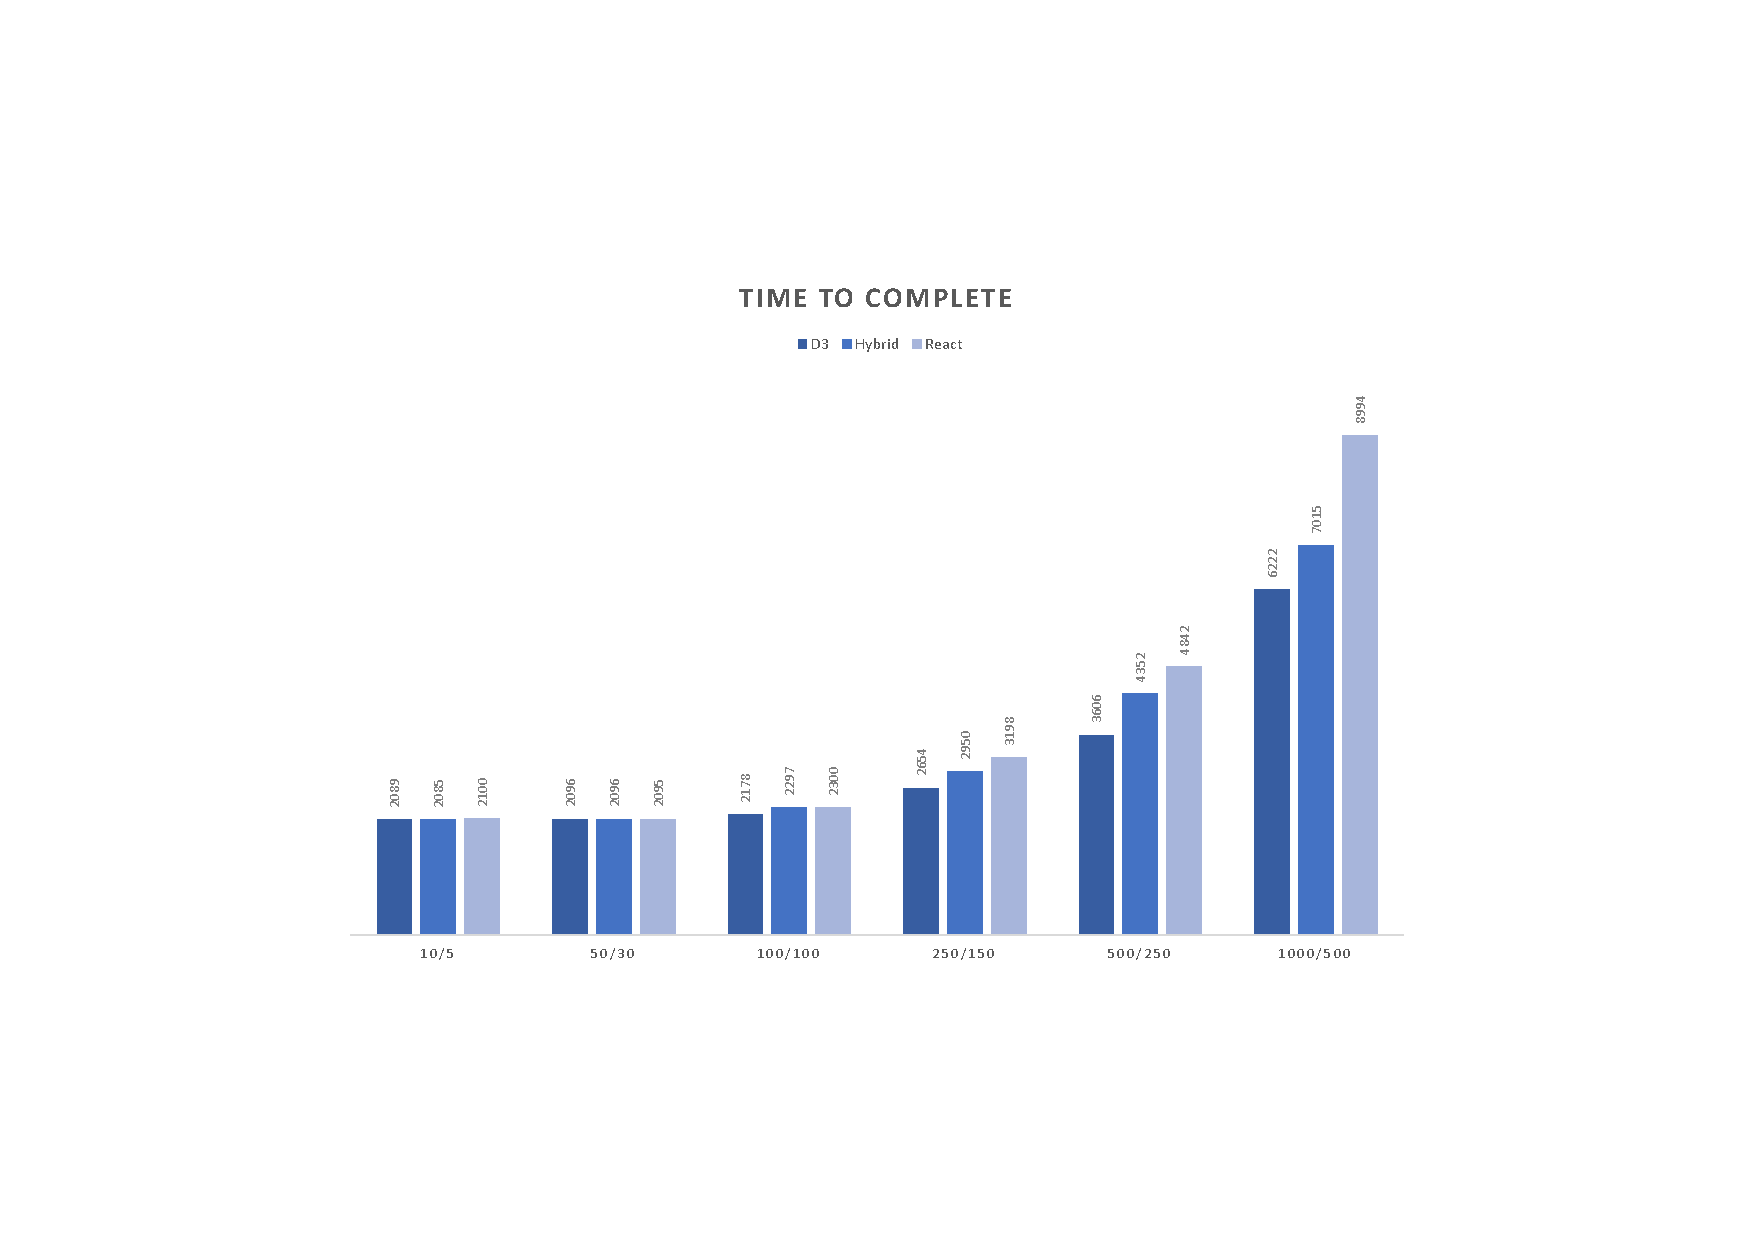
\includegraphics[scale=2.5, trim= 4cm 4.5cm 4cm 4.5cm, clip, width=1\columnwidth]{perfHighEnd002.pdf}
\caption{High-end devices' average time to complete for one benchmark iteration cycle in milliseconds (lower is better).}
\label{fig:perfHighEnd002}
\end{figure}

%% frametime another way to display frames per second, just another calculation

Measuring the average frame time of animations can provide insights into the user's perception of fluid animation. If the value is too high, the animation may not be experienced as a smooth animation. Therefore measuring the value is crucial when comparing the prototypes to each other. Figure \ref{fig:perfLowEnd003} shows a bar chart of the low-end device benchmark. Towards the last two iterations, the benchmark configuration seems to have hit a certain threshold since the values rise exponentially. The other performance result shows a similar pattern to the previous results, however.

\begin{figure}
\centering
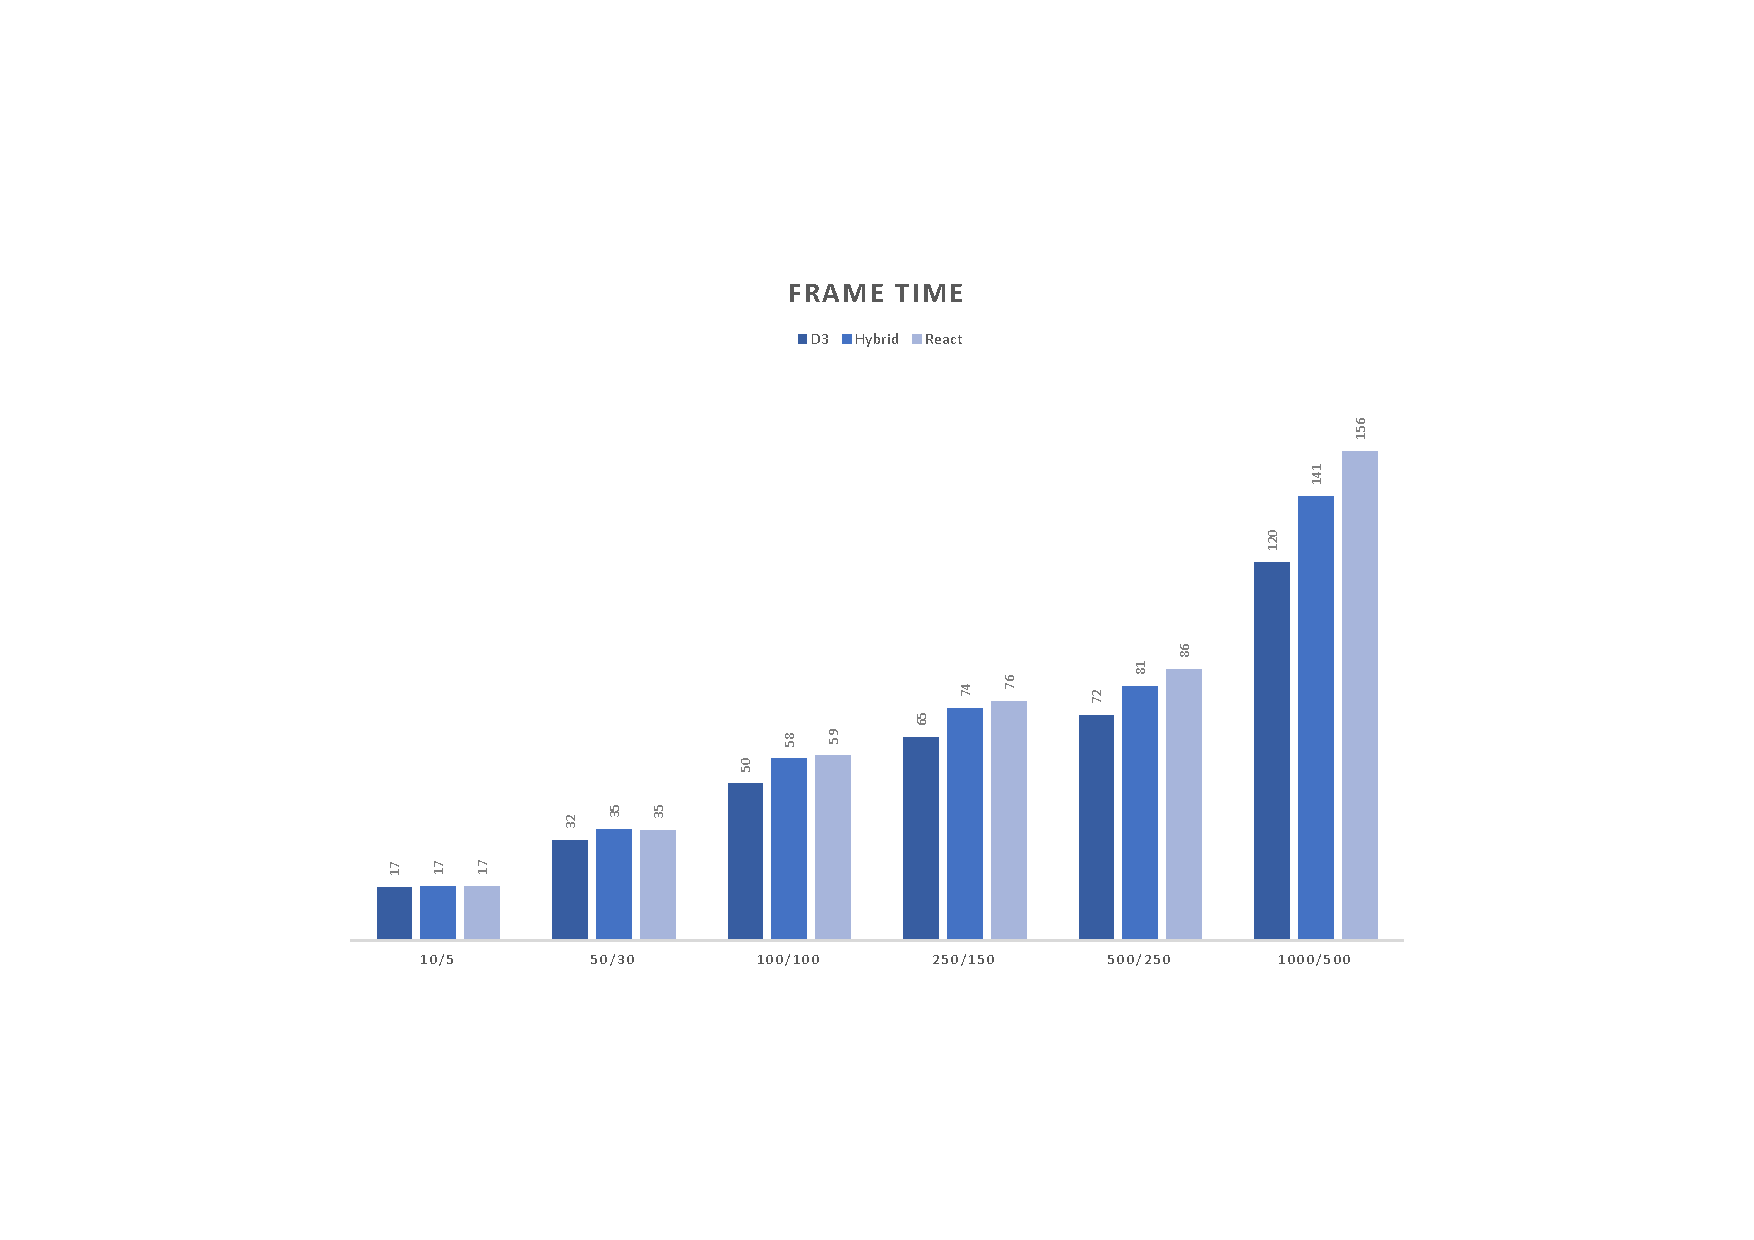
\includegraphics[scale=2.5, trim= 4cm 4.5cm 4cm 4.5cm, clip, width=1\columnwidth]{perfLowEnd003.pdf}
\caption{Low-end devices' average frame time per benchmark iteration cycle (lower is better).}
\label{fig:perfLowEnd003}
\end{figure}

Looking at the high-end results in figure \ref{fig:perfHighEnd003} the same problem as before can be observed, where the first iterations are capped to a specific minimum value. However, the rest of the results increase exponentially, which correlates to the rest of the high-end performance results. The average frame time of the last iteration breaks out and spikes with an exceptionally high value.

\begin{figure}
\centering
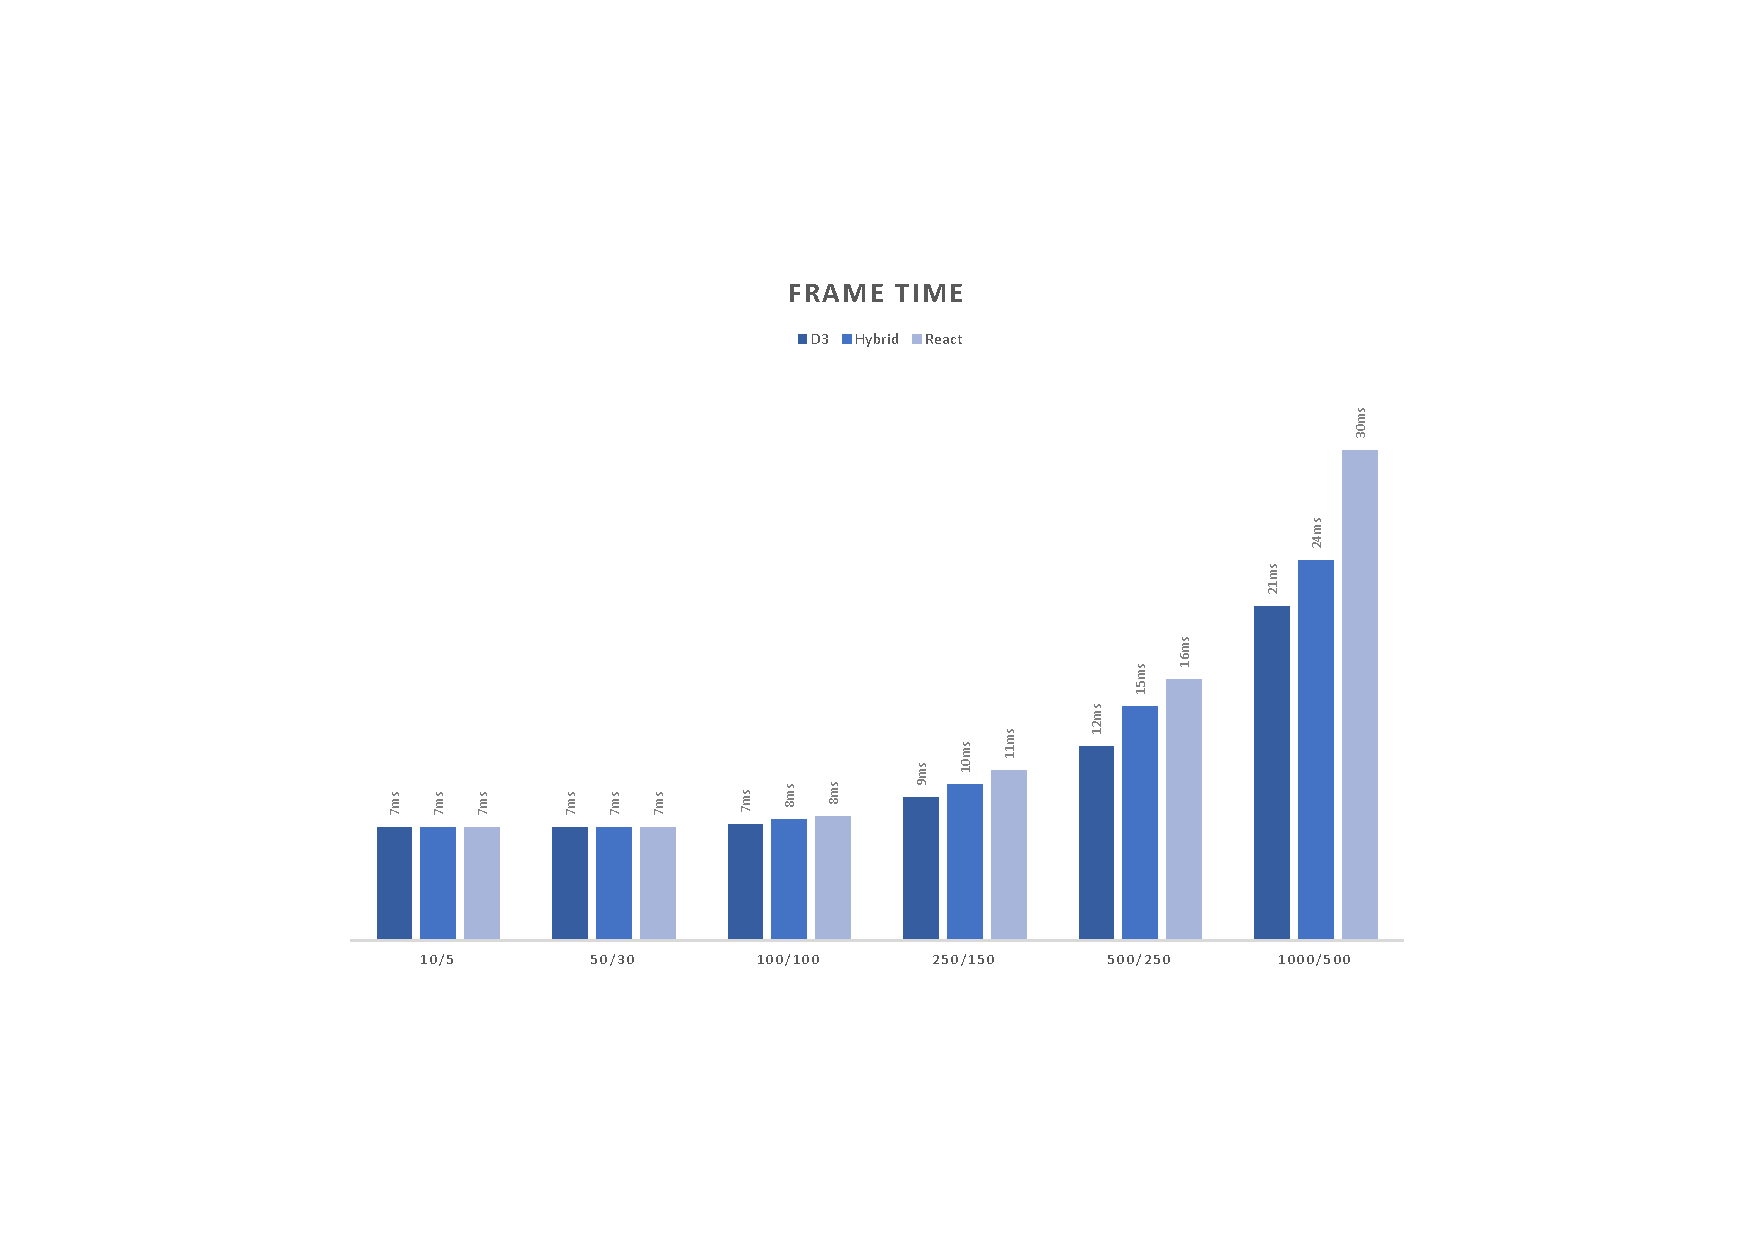
\includegraphics[scale=2.5, trim= 4cm 4.5cm 4cm 4.5cm, clip, width=1\columnwidth]{perfHighEnd003.pdf}
\caption{High-end devices' average frame time per benchmark iteration cycle (lower is better).}
\label{fig:perfHighEnd003}
\end{figure}

Last but not least, a critical aspect of any animation performance measurement is the maximum time between frames measured. The value can provide critical insights to some performance issues even though the average frame time per second might look okay. The chart in figure \ref{fig:perfLowEnd004} shows an average of the maximum frame time value to each iteration cycle. One unanticipated result was that the maximum frame rate of the hybrid component is significantly higher throughout the testing results than the pure D3 or pure React components.

\begin{figure}
\centering
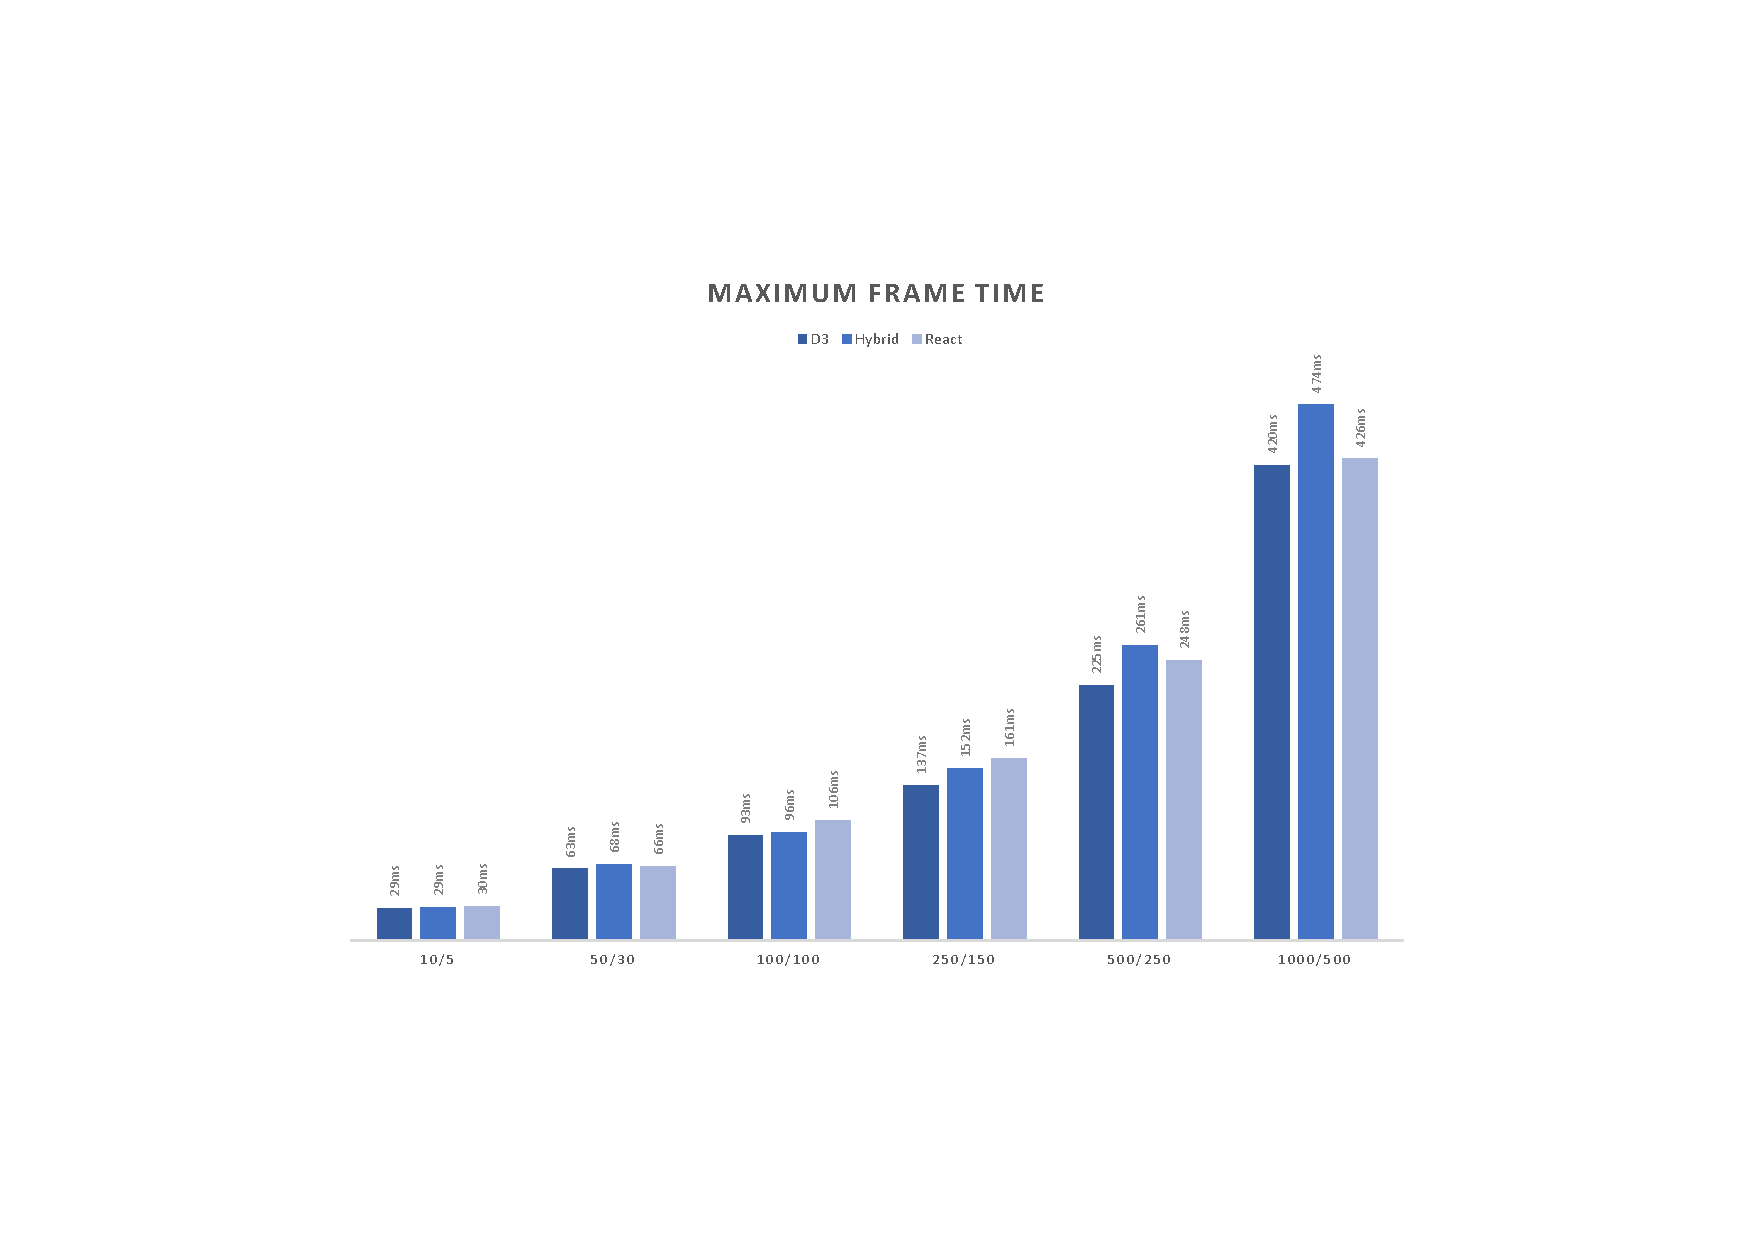
\includegraphics[scale=2.5, trim= 4cm 4.5cm 4cm 4.5cm, clip, width=1\columnwidth]{perfLowEnd004.pdf}
\caption{Low-end devices' average maximum frame time per benchmark iteration cycle (lower is better).}
\label{fig:perfLowEnd004}
\end{figure}

However, the performance graph in figure \ref{fig:perfHighEnd004} shows more expected results. Again, the average maximum frame time rises exponentially. The results contain a few irregularities, though. The maximum frame time of the reference pure D3 prototype, for example, is sometimes higher as the value of the other two prototypes. The maximum frame time values, therefore, must be taken with a grain of salt, as any maximum value could be falsified by an unexpected system or browser activity which could have decreased the overall performance of any prototype. As mentioned before, the problem is mitigated by executing one iteration multiple times, but there is still a margin of error, though.

\begin{figure}
\centering
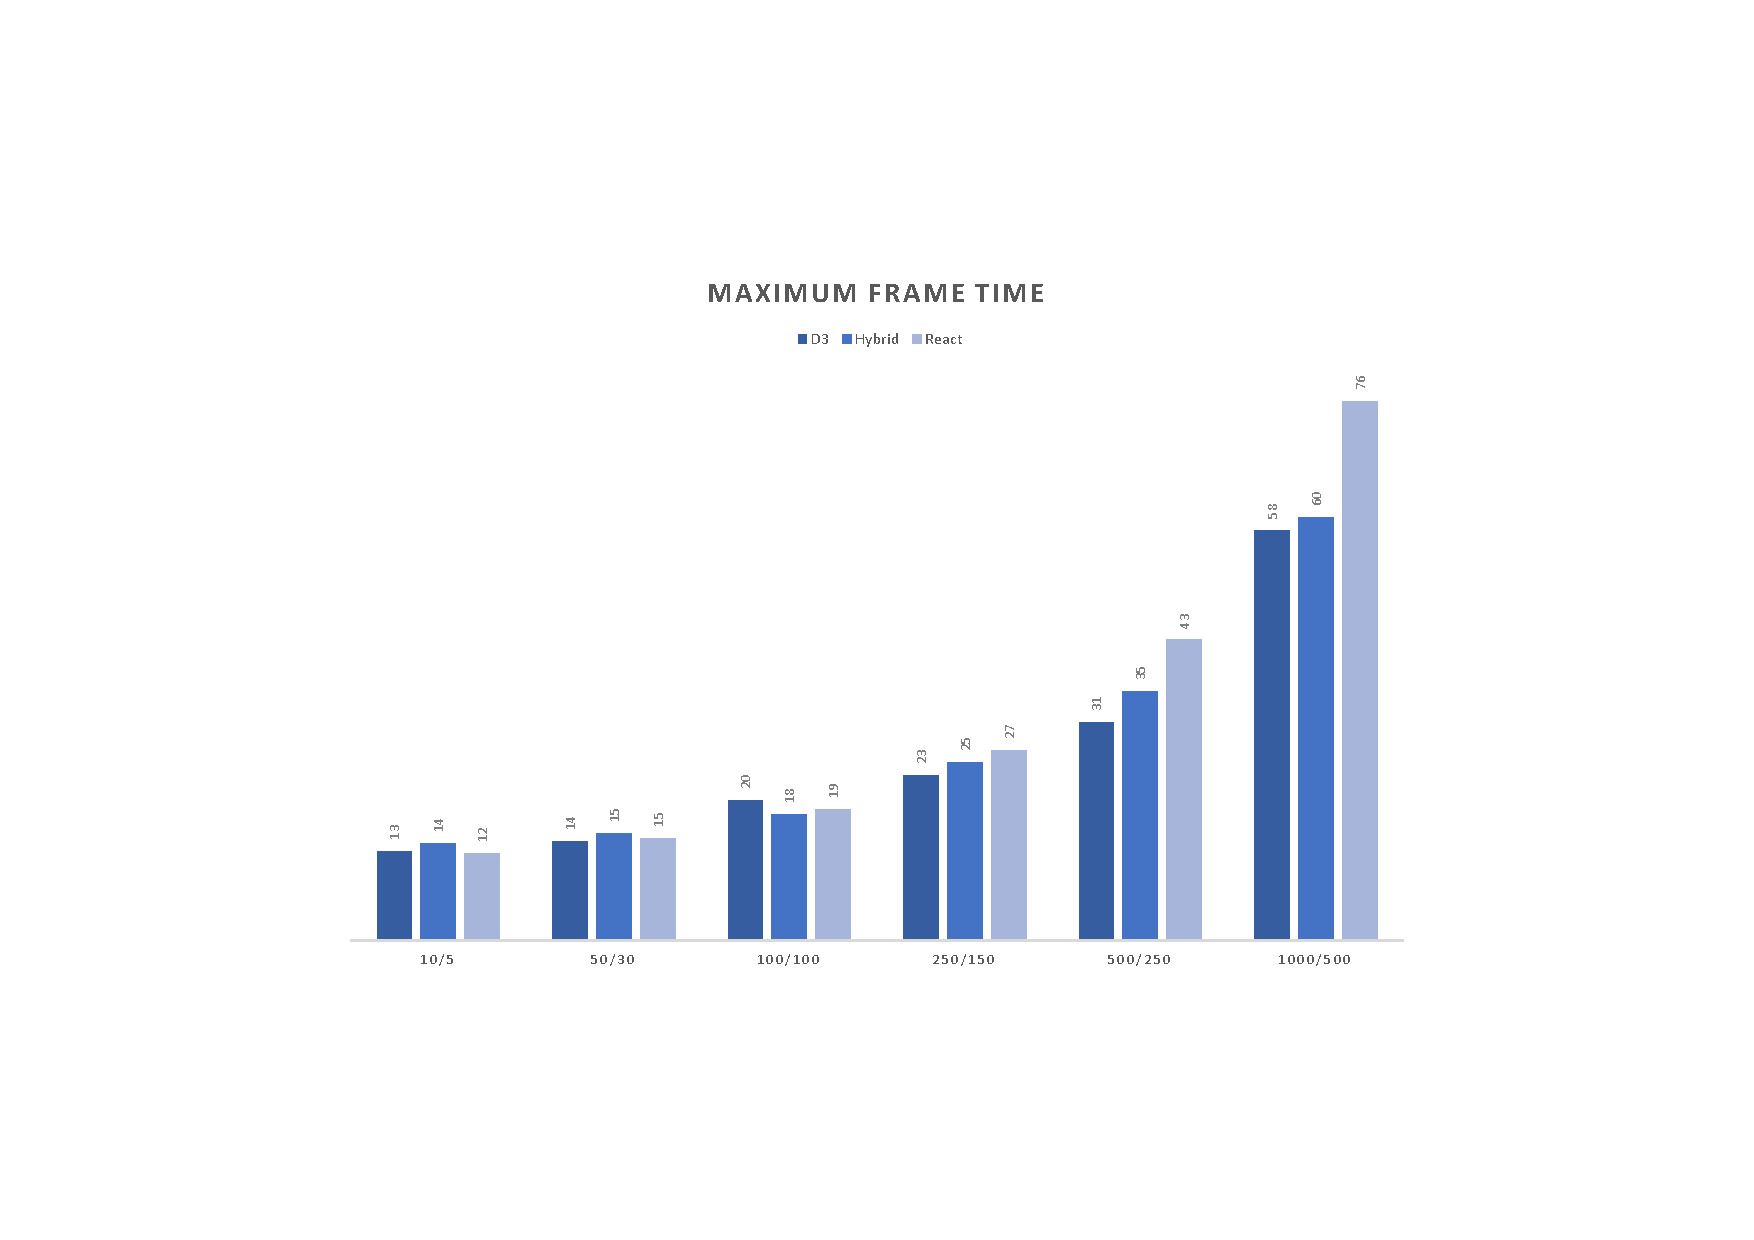
\includegraphics[scale=2.5, trim= 4cm 4.5cm 4cm 4.5cm, clip, width=1\columnwidth]{perfHighEnd004.pdf}
\caption{High-end devices' average maximum frame time per benchmark iteration cycle (lower is better).}
\label{fig:perfHighEnd004}
\end{figure}

\subsection{Human Perception of Fluid Animations}
\label{sub:humanPerception}

%%Humans vision is bad lol, they can only see 13 FPS but when do we actually notice some stuttering or laggy animation performance? 

Human vision is a very complicated topic, as there has been a large volume of studies for years which tried to determine at which point humans perceive a series of images as fluid motion. The article in \cite{RestorationOfMotionPictureFilm} claims that humans perceive motion if the animation is displayed with at least 12 frames per second. During further research, another article was found which states that humans can detect specific images in a rapid serial visual representation (RSVP) of a series of multiple pictures. The paper in \cite{Potter2014} found that participants could determine if the RSVP stream contained a specific picture even with a frequency of displaying each picture for just 13ms. 

Another vital question is at which point an observer does not perceive an animation as fluid anymore. As mentioned before, the time per frame should be below 13ms in the best case to provide the perception of fluid animation. Although animations with at least 12 frames per second can be perceived as motion, they are not necessarily experienced as fluid motion though. As the performance measurements of the thesis project yield some final numbers, they can be used to determine if the animation of the test can be experienced as fluid motion or not.

Further research in the field of human perception of animation revealed yet another interesting result. Countless studies throughout the last decades have tried to find an answer to the question at which point humans do not experience an animation as stuttering or flickering anymore. The answer of most research papers is, though that flickering or so-called "stuttering" cannot be detected if the human perception cannot distinguish between modulated light and a stable field anymore. After doing some extensive research, the rate seems to be between 50 and 90 Hertz according to several papers like \cite{6375944}, \cite{farrell1987predicting} or \cite{stereoscopicFlickerArticle}. The papers are mostly about the monitors' refresh rate, but the same also applies for the displayed frames per second of an animation rendered in the browser.

\subsection{Interpreting the Test Results}

When interpreting the test results, it is essential to keep in mind that the hybrid implementation uses a custom animation library internally, as mentioned in subsection \ref{sub:D3AndReactHybrid} which can be turned off to improve performance. The animation feature was turned on during the execution of the benchmark tests even though the test iterations do not include any individual node animation. As a result, the pure React component has a clear advantage over the hybrid component by not having to calculate node animations as they are not implemented on the pure React component. Even though the additional performance decreasing feature was kept on during all tests, the hybrid component generally yielded equal or better performance numbers in comparison to the pure React prototype.

Another clear advantage of the React prototype is that newer versions of React provide functionality which assigns a lower priority to DOM nodes which are outside the viewport of the browser. Lin Clark explains the functionality of the library during the React conference in \cite{ReactReconcliliationVideo}, where the feature was first introduced. Due to the fact that mobile devices mostly have smaller viewports, a large proportion of the nodes in higher iteration difficulties is rendered outside of the viewport again providing an advantage to the React prototype.

Looking at the frames per seconds, the charts in figures \ref{fig:perfLowEnd001} and \ref{fig:perfHighEnd002} indicate how the D3 prototype yields the best result in every iteration, followed by the hybrid implementation with the second best results and lastly the pure React prototype with the slowest results. Closer inspection of the two charts shows that the performance decrease is linear, whereas the increase of render difficulty in figure \ref{fig:perfIterations} is exponential. Because the frames per second are calculated via the \texttt{requestAnimationFrame()} function, the results show that the browsers regularly try to provide animation frames even though the calculations get exponentially harder.

In comparison to the earlier presented results, the overall time to complete values in the charts in figures \ref{fig:perfLowEnd002} and \ref{fig:perfHighEnd002} do not correlate to the frames per second which is a rather unexpected result. Like mentioned before, browsers try to provide as many animation frames as possible, whereas the overall time to complete is measured via two timestamps. A remarkable outcome though is the fact that the first and most lightweight iteration results show that the low-end devices' time to complete is roughly 40\% of the high-end devices' time to complete. This supports the theory that the monitor refresh rate is directly tied to the browsers' request animation frame functionality as 40\% of 144 roughly equals 60. 

The high-end and low-end time to complete values do not correlate either. While the high-end benchmark values in figure \ref{fig:perfHighEnd002} show the expected exponential increase of time to complete, the low-end results in figure \ref{fig:perfLowEnd002} show a linear increase for the time to complete one iteration cycle. The findings can be explained that browsers cannot complete full render and paint cycles anymore during one animation frame due to the low-end hardware. By generating a constant backlog of due animation frames, some of them might get dropped due to new animation frame requests that are more recent. Once animation frames get canceled because of more recently requested animation frames, the pattern of increasing completion time is more comparable to the pattern the overall FPS increase in the charts in figures \ref{fig:perfLowEnd001} and \ref{fig:perfHighEnd002}. The high-end results in figure \ref{fig:perfHighEnd002} show the expected exponential increase of time to complete an iteration cycle, as browsers can process the calculations completely within the requested animation frame.

Figures \ref{fig:perfLowEnd003} and \ref{fig:perfHighEnd003} show the average frame times of the prototypes. The results can be seen as another way to describe frames per second. As described in section \ref{sub:humanPerception}, the frame times play a crucial role for humans to percept an animation as fluid without stuttering. Near all low-end device, benchmarks showed a rather high average frame times starting from the second benchmark iteration. While the results stayed well above the previously mentioned 12 frames per second threshold, the lower frame time is definitely noticeable. Probably one of the most significant findings when looking at the general trend, the hybrid prototype regularly comes out ahead, when comparing the average frame times. The high-end chart in figure \ref{fig:perfHighEnd003} shows a clear spike of the pure React implementation in the last iteration. A possible explanation for this outcome might be that React reaches the previously already mentioned threshold when performing the calculation for an animation frame. React performs pretty well, considering it has to process 1500 DOM nodes every 30ms completely and put them through a complete render cycle.

Last but not least, the maximum frame time results can also provide valuable insights into how the prototypes perform compared to each other. These results must be interpreted with caution, though because various unforeseeable reasons can cause maximum frame time spikes. The results for the low-end devices in figure \ref{fig:perfLowEnd004} show, for example, that the hybrid component had the highest maximum frame time in the last two iterations. Now, if this only happens once in the animation, this might not be noticeable, but if this would be a continuous trend, the data could point to a performance problem in the implementation of the prototype. The explanation to the performance spikes is most likely also tied to the fact that low-end devices run into the animation frame limit of not being able to calculate a full render cycle in one animation frame. The hybrid component not only has to build up the whole component tree via react but also calculate the animations with react move. If both instances are limited to animation frame constraints, the calculation could be spread out across multiple frames, making the whole animation slower in the process.

On the contrary, the high-end maximum frame time tests in figure \ref{fig:perfHighEnd004} yield more expected results. When having to deal with many nodes and links, the maximum frame times should be equally affected as a consequence. The last iteration shows the longest time between frames for the pure React prototype, which is 76 milliseconds. The pure React and hybrid component seem to be able to maintain a maximum frame time at about 60 milliseconds equally.

%Generally a correlation between the time to complete, average frame time and the maximum frame time can be observed when looking at all the charts again.

\section{Conclusion}

All in all, the different prototypes performed quite well in general. The question "Why does the benchmark use as high numbers like 1000 nodes and 500 links?" which might come up during the examination of the testing results can quickly be answered. The test that was used to benchmark the prototypes uses a simple force simulation configuration where each base node is just a single circle element, and each link is a path element. When using more sophisticated nodes which contain multiple SVG elements, the outcome could be the same. If an example simulation would use 10 SVG elements in just one node, when rendering 100 nodes the outcome would yield a similar outcome as rendering the 6th iteration of the benchmarks with 1000 nodes and 500 links.

Overall all the prototypes performed pretty well. As mentioned before, the pure D3 component is the clear winner and best performing prototype, but that was the expected result, as it was developed to serve as a baseline for the results of the other prototypes. When glancing over the rest of the results, the hybrid nearly always comes out ahead of the pure React prototype. The primary purpose of the study was if React can be combined with D3 without losing performance in the browser. The definitive answer to that question has to be no, unfortunately, as there are some performance penalties when combining two full grown libraries. The test results also support the answer to the research question.

When talking about user experience though, the prototypes are pretty much all usable in production projects, as the divergence of the performance numbers mostly stays within the bounds of a smooth animation experience. The benchmark results of the third and fourth iteration are acceptable when looking at the FPS and average frame time. When using the force graphs on mobile devices, the performance is worse overall, but due to the fact that even the pure D3 prototypes performed a lot worse on low-end devices, the combination prototypes cannot magically yield a better performance, as they technically not only have to calculate D3 force simulation ticks but also React render cycles. As a consequence, the performance is worse than just letting D3 handle the whole simulation on its own. 


\chapter{Open Source and the React Community}
\label{cha:opensource}

Ultimately the thesis project was always planned to be an open source project at some point in the future. The current React community is extremely active and productive because of countless open source projects that provide useful libraries that can be used in every project free of charge. As the thesis project is quite the success in terms of the achieved goals and the performance numbers, the overall result should not only be presented in this masters' thesis. Instead the project should be published to the React community who truly benefits from the software.

This chapter is about the publishing plans of the hybrid prototype and what API it should have to provide the most benefit to the users of the component. The thesis project was created out of necessity for a component that would handle a D3 force simulation but can be written in React code. The first versions of the API will probably be very opinionated, as there was a special usecase for the component. Maybe the community will alter the proposed component API in the future though.

\section{Building an Open Source Library Component}

Conceptionally speaking, if there is a library that ships a single component, the React component has to be somehow packaged and then published to npm\footnote{https://www.npmjs.com/} to be usable by other developers. Since npm is one of the biggest package manager for web projects, the component can be installed in any web project once it has been published to the npm registry. Bundler tools like webpack\footnote{https://webpack.js.org/}, rollup\footnote{https://rollupjs.org}, or parcel\footnote{https://parceljs.org/} make it easy to create static library assets that can be published to npm.

Furthermore, the code should be hosted on a public collaboration platform. The best option to host a public VCS repository is GitHub\footnote{https://github.com/} of course, as public projects can be hosted free of charge. As a consequence the ultimate goal of opensourcing the component is to not only publish the component to npm but also to GitHub. Most if not almost all of the open source third party react component code bases are hosted on GitHub.

The usage of the react component should be as easy and straigt forward as possible to enable developers an easy starting point to using the component. The API should be designed in a way that programmers can incrementally opt into more complicated features. By simply using the component with the standard required props, a standard D3 force simulation should be rendered. After going through the documentation and the tutorial, developers should also be able to gracefully opt into the more complicated features of the component like custom node and link rendering.

As mentioned in section \ref{subsub:hybridDisadvantages}, a big disadvantage of the hybrid component is the fact that developers must understand how the hybrid implementation works in order to being able to start contributing to the open source component. The library should therefore have a very elaborated and well written contribution documentation to make it easier to contribute to the component.

\section{Technical Details of the Component API}

\begin{program}
\caption{Alpha version of the force graph component API}
\label{prog:hybridForceGraphComponentAPI}
\begin{JsCode}
<HybridForceGraph 
  height={height}
  width={width}
  nodes={nodes}
  links={links}
  forceOptions={simulationOptions} /+\label{line:foceOptions}+/ /+\label{line:optional}+/ 
  nodeTickHandler={nodeTickHandler}
  renderNode={customNodeRenderer}
  renderLink={customLinkRenderer}
  animation={animationConfig}
/>
\end{JsCode}
\end{program}

A draft version of the API was already implemented throught the implementation phase of the master thesis project. The storybook already utilizes the API to show customized versions of the hybrid force graph. The program in \ref{prog:hybridForceGraphComponentAPI} shows, how the component API looks like. There are a few mandatory props like the height and width of the SVG element. The nodes and links could be omitted, but it wouldn't make any sense, as the force graph has to get its data from somewhere. The two data properties are designed to take falsey values in case the data comes from a web API and is not available during the first parent component render cycle. Every prop starting on line \ref{line:optional} and onwards is optional and can be fully customized by the user of the component.

In chapter \ref{cha:visualization} the figure \ref{fig:reactD3stroy} shows a component story of a customized force graph component. The snippet in \ref{prog:customForceGraph} shows the sourcecode for the custom component. Instead of using the default node renderer, a custom node rendering function is used as it can be seen on lines \ref{line:customNodeRenderer} and \ref{line:useCustomNodeRenderer}. The custom node renderer renders a base \texttt{<g>} SVG element per node, which contains three circles with different radius settings. 

Due to the fact that the base element is not a circle element anymore, the ticking function has to be customized as well. Line \ref{line:customTickHandler} in \ref{prog:customForceGraph} shows the implementation of the custom tick handler. Instead of passing the position via \texttt{cx} and \texttt{cy} coordinates, the function applies a transform property to the the node selection which translates the base node to the x and y coordinates. The translation is necessary, as the group SVG element cannot directly accept x and y coordinates.

\begin{program}
\caption{Alpha version of the force graph component API}
\label{prog:customForceGraph}
\begin{JsCode}
const customTickHandler = (nodeSel) => /+\label{line:customTickHandler}+/ 
  nodeSel.attr('transform', ({ x, y }) => `translate(${x},${y})`)

const customNodeRenderer = ({ id, size }) => ( /+\label{line:customNodeRenderer}+/ 
  <g id={id} key={id} className={'node'}>
    <circle r={size} fill={'lightblue'} />
    <circle r={size - 5} fill={'pink'} />
    <circle r={size - 10} fill={'palevioletred'} />
  </g>
)

const CustomForceGraph = ({ height, width, nodes, links }) => (
  <HybridForceGraph
    height={height}
    width={width}
    nodes={nodes}
    links={links}
    nodeTickHandler={customTickHandler}
    renderNode={customNodeRenderer} /+\label{line:useCustomNodeRenderer}+/ 
    animation={null}
  />
)
\end{JsCode}
\end{program}

The code example in \ref{prog:customForceGraph} demonstrates really well, how the graceful opt-in strategy of the API works. The example does not use every possible prop that can be added to the force graph like demonstrated in the code example in \ref{prog:hybridForceGraphComponentAPI}. The implementation of the custom graph omits the \texttt{forceOptions} prop for example. The hybrid force graph component falls back to the standard force simulation configuration as a result. The custom link render function prop is also omitted as the default link implementation is sufficient for the custom force graph.

\section{Final Thoughts}

In the end only time will tell, if the component is useful for the community once it is published and if there are some open source developers willing to contribute to the project. Due to fact that the force graph component is already utilized in at least one production project the library component is already a success.
\chapter{Conclusion}
\label{cha:conclusion}

%%%----------------------------------------------------------
%\appendix                                         % appendix 
%%%%----------------------------------------------------------
%
%\chapter{Technical Details}
\label{app:TechnicalDetails}



	% technical supplements
%\chapter{CD-ROM Contents}
\label{app:cdrom}

\paragraph{Format:} 
CD-ROM, Single Layer%

\section{Master's Thesis}
\dirtree{%
  .1 /.
  .2 thesis.
  .3 latex-source\DTcomment{latex source files}.
  .3 online-references\DTcomment{snapshots of online references}.
  .3 thesis\_EN.pdf\DTcomment{master's thesis (main document)}.
  .3 benchmark-results.xlsx\DTcomment{excel file containing all results and calcluations}.
}

\section{Thesis Project -- Combining React and D3}
\dirtree{%
.1 /.
.2 combining-react-and-d3.
.3 .storybook\DTcomment{storybook config files}.
.3 public\DTcomment{publicly served files}.
.3 src\DTcomment{application source}.
.4 assets\DTcomment{static assets}.
.4 components\DTcomment{prototypes and generic app components}.
.4 lib\DTcomment{utility functions}.
.4 pages\DTcomment{application pages}.
.4 stories\DTcomment{storybook stories}.
.4 app.js\DTcomment{root application file}.
.4 index.js\DTcomment{index file}.
.4 routes.js\DTcomment{application route configuration}.
.4 serviceWorker.js\DTcomment{service worker configuration}.
.3 *\DTcomment{config files}.
}
	% contents of the CD-ROM/DVD
%\chapter{Questionnaire}
\label{app:Questionnaire}





	% chronological list of changes
%\chapter{\latex Source Code}
\label{app:SourceCode}

	% source text of this document

%%%----------------------------------------------------------
\MakeBibliography                        				% references
%%%----------------------------------------------------------

%%% special page for checking print size --------------------
\chapter*{Check Final Print Size}

\begin{center}
{\Large --- Check final print size! ---}

\bigskip

\calibrationbox{100}{50} % width/height of box in mm

\bigskip

{\Large --- Remove this page after printing! ---}

\end{center}



%%%----------------------------------------------------------
\end{document}
%%%----------------------------------------------------------